%% This is file `DEMO-TUDaReport.tex' version 3.16 (2021/06/03),
%% it is part of
%% TUDa-CI -- Corporate Design for TU Darmstadt
%% ----------------------------------------------------------------------------
%%
%%  Copyright (C) 2018--2021 by Marei Peischl <marei@peitex.de>
%%
%% ============================================================================
%% This work may be distributed and/or modified under the
%% conditions of the LaTeX Project Public License, either version 1.3c
%% of this license or (at your option) any later version.
%% The latest version of this license is in
%% http://www.latex-project.org/lppl.txt
%% and version 1.3c or later is part of all distributions of LaTeX
%% version 2008/05/04 or later.
%%
%% This work has the LPPL maintenance status `maintained'.
%%
%% The Current Maintainers of this work are
%%   Marei Peischl <tuda-ci@peitex.de>
%%   Markus Lazanowski <latex@ce.tu-darmstadt.de>
%%
%% The development respository can be found at
%% https://github.com/tudace/tuda_latex_templates
%% Please use the issue tracker for feedback!
%%
%% If you need a compiled version of this document, have a look at
%% http://mirror.ctan.org/macros/latex/contrib/tuda-ci/doc
%% or at the documentation directory of this package (if installed)
%% <path to your LaTeX distribution>/doc/latex/tuda-ci
%% ============================================================================
%%
% !TeX program = lualatex
%%

\documentclass[
	ngerman,
	accentcolor=9c,% Farbe für Hervorhebungen auf Basis der Deklarationen in den
	type=intern,
	marginpar=false
	]{tudapub}

\usepackage[english, main=ngerman]{babel}
\usepackage[autostyle]{csquotes}
\usepackage{amsmath}
\usepackage{amssymb}
\usepackage{tikz}
\usetikzlibrary{tikzmark,calc}
\usepackage{graphicx}
\usepackage{amsfonts}
\usepackage{enumitem}
\usepackage{mathtools}
\usepackage{mathrsfs}
\DeclarePairedDelimiter\ceil{\lceil}{\rceil}
\DeclarePairedDelimiter\floor{\lfloor}{\rfloor}

\graphicspath{ {./images/} }

%Formatierungen für Beispiele in diesem Dokument. Im Allgemeinen nicht notwendig!
\let\file\texttt
\let\code\texttt
\let\pck\textsf
\let\cls\textsf

\begin{document}
\newtheorem{satz}{Satz}[section]
\numberwithin{satz}{subsection}
\newtheorem{korolar}[satz]{Korolar}
\newtheorem{definition}[satz]{Definition}





\title{Mathe III Formelsammlung}
\author{Luca Liontos}
%\date{} % Ohne Angabe wird automatisch das heutige Datum eingefügt

\maketitle

\tableofcontents
\newpage

\section{Interpolation}
    \subsection{Polynominterpolation}
        n = Anzahl Stützstellen - 1
        \subsubsection{Lagrange}
            \begin{equation*}
                 \begin{array}{l c r}
                             p_n(x) = \sum_{k=0}^n y_k L_{k,n}(x) & \text{mit} & L_{k,n} (x) = \prod_{\substack{j=0 \\ j\not=k}}^n \dfrac{x-x_j}{x_k-x_j}
                \end{array}
            \end{equation*}
            \textbf{Trick effiziente/ übersichtliche Berechnung}\\
            \begin{center}
                \begin{tabular}{c || c | c | c | c | c |}
                    k/j & $x_0$ & $x_1$ & \dots & $x_n$ & $L_{k,n}$\\
                    \hline
                    \hline
                    $x_0$ & $\backslash$ & $\dfrac{x-x_1}{x_0-x_1}$ & \dots & $\dfrac{x-x_n}{x_0-x_n}$ & $\prod\text{diese Zeile}$\\
                    $x_1$ & $\dfrac{x-x_0}{x_1-x_1}$ & $\backslash$ & \dots & $\dfrac{x-x_n}{x_1-x_n}$ & $\prod\text{diese Zeile}$\\
                    $\vdots$ & $\vdots$ & $\vdots$ & $\ddots$ & $\vdots$ & $\vdots$\\ 
                    $x_n$ & $\dfrac{x-x_0}{x_n-x_0}$ & $\dfrac{x-x_1}{x_n-x_0}$ & \dots & $\backslash$ & $\prod\text{diese Zeile}$
                \end{tabular}
            \end{center}
        \begin{satz}
                es gibt genau ein Polynom $p(x)$ vom Grad $\leq n$, das die Interpolationsbedingungen erfüllt, nämlich $p_n(x)$
        \end{satz}
       \subsubsection{Newton}
        \begin{equation*}
            \begin{array}{cc}
                p_n(x) = \gamma_0 + \sum_{i=1}^{n} \gamma_i (x-x_0) \dots (x-x_{i-1}), & \gamma_i = f_{[x_0 \dots x_i]}    
            \end{array}
        \end{equation*}
        \begin{equation*}
            f_{[x_j,\dots,x_{k+j}]} = \dfrac{f_{[x_{j+1} \dots, x_{j+k}]} - f_{[x_{j} \dots, x_{j+k-1}]}}{x_{j+k} - x_j} = \dfrac{f_{\text{unten}} - f_{\text{oben}}}{x_{\text{unten}} - x_{\text{oben}}}
        \end{equation*}
        Die oberste Zeile ab dem Strich sind dann die $\gamma_i$
        \begin{center}
            \begin{tabular}{c | c c c}
                $x_0$   & $f_{[x_0]} = y_0$ \tikzmark{0}  &                  & \\
                        &                   & \tikzmark{01l} $f_{[x_0,x_1]}$ \tikzmark{01r} & \\
                $x_1$   & $f_{[x_1]} = y_1$ \tikzmark{1}  &                  & \tikzmark{012}$f_{[x_0,x_1,x_2]}$\\
                        &                   & \tikzmark{12l} $f_{[x_1,x_2]}$ \tikzmark{12r} & \\
                $x_2$   & $f_{[x_2]} = y_2$ \tikzmark{2}  &                  & \\
                $\vdots$&                   &                                & \\
            \end{tabular}
        \end{center}
        \begin{tikzpicture}[overlay,remember picture,shorten >=5pt,shorten <=1pt]
                            \draw [->] ({pic cs:0}) -- ({pic cs:01l});
                            \draw [->] ({pic cs:1}) -- ({pic cs:01l});
                            \draw [->] ({pic cs:1}) -- ({pic cs:12l});
                            \draw [->] ({pic cs:2}) -- ({pic cs:12l});
                            \draw [->] ({pic cs:01r}) -- ({pic cs:012});
                            \draw [->] ({pic cs:12r}) -- ({pic cs:012});
        \end{tikzpicture}
        %\begin{figure}[ht]
        %    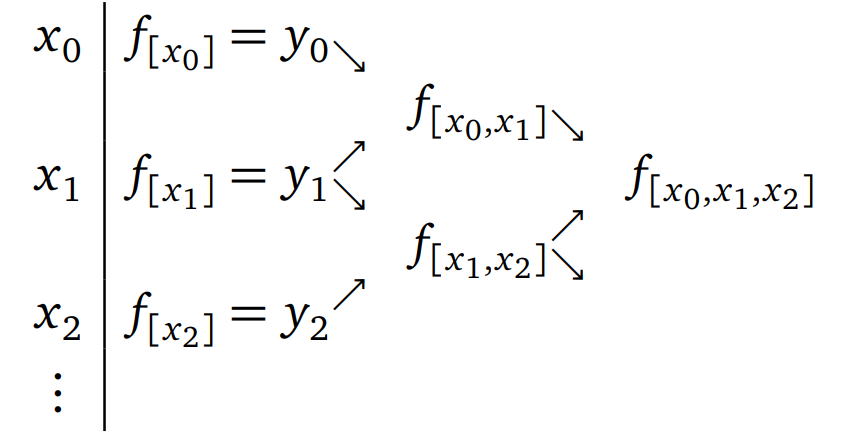
\includegraphics[scale=0.3]{images/grafik.png}
        %    \centering
        %\end{figure}
       Hinweis: Man kann Zeilen vertauschen. Das heißt wenn viele $f_{[x]} = 0$ lohnt es sich meist diese nach oben zu tauschen.

       \subsubsection{Fehlerabschätzung}
       \setcounter{satz}{2}
       \begin{satz}
            Voraussetzungen für max error Korolar: f ist n+1 mal stetig diffbar
       \end{satz}
       \begin{korolar} 
            
            Wenn Satz 1.1.3 gilt:\\
            \textbf{Äquidistant}:
            \begin{equation*}
                \max_{x \in [a,b]} |f(x) - p_n(x)| \leq \max_{x \in [a,b]} \dfrac{|f^{(n+1)}(x)|}{(n+1)!}(b-a)^{n+1}
            \end{equation*}
            \textbf{Tschebyschev-Abszissen}:
            \begin{equation*}
                \max_{x \in [a,b]} |f(x) - p_n(x)| \leq \max_{x \in [a,b]} \dfrac{|f^{(n+1)}(x)|}{(n+1)!}\left(\dfrac{b-a}{2}\right)^{n+1}2^{-n}
            \end{equation*}
       \end{korolar}
       \textbf{Inverse Interpolation}:\\
       Sei $f:[a,b] \rightarrow \mathbb{R}$ bijektiv.
       Sind dann alle $(x_i,y_i), y_i = f(x_i)$ Stützpunkte von $f$
       dann sind $(y_i, x_i)$ Stützpunkte für $f^{-1}$ und eine Approximation kann durch Interpolation dieser
       gewonnen werden.


       Hinweis:\\
       $f$ ist auf Wertebereich von $x$ stetig differenzierbar und aufgrund der Ableitung streng monoton wachsend $\Rightarrow$ injektiv\\
       Die Grenzen von x müssen genau  auf die Grenzen von y abbilden, da dann (wegen monoton wachsend) die gesamte Zielmenge getroffen wird $\Rightarrow$ surjektiv\\
       $\Rightarrow$ bijektiv

       \subsection{Spline-Interpolation}
            \begin{definition}
                Eine Splinefunktion der Ordnung $k$ zur Zerlegung $\Delta$ ist eine Funktion $s:[a,b]\rightarrow \mathbb{R}$ mit folgenden Eigenschaften:
                \begin{itemize}
                    \item es gilt $s \in C^{k-1}([a,b])$ (stetig diffbar)
                    \item s stimmt auf jedem Intervall $[x_i,x_{i+1}]$
                \end{itemize}
                \textbf{Spline-Interpolation}: \\
                Zu einer Zerlegung $\Delta = \{x_i:a = x_0 < x_1 < \dots < x_n = b\}$ und werten $y_i \in \mathbb{R}, i = 0, \dots, n$
                bestimme $s \in S_{\Delta,k}$ mit
                \begin{equation*}
                    s(x_i) = y_i, i=0,...,n
                \end{equation*}
            \end{definition}
            \subsubsection{Linear}
                \begin{equation*}
                    s(x) = s_i(x) = \dfrac{x_{i+1} - x}{x_{i+1} - x_i} y_i + \dfrac{x - x_{i}}{x_{i+1} - x_i} y_{i+1} \mbox{ }\forall x \in [x_i, x_{i+1}]
                \end{equation*}
                mit Hilfsknoten $x_{-1} < a $ und $ x_{n+1} > b$ gilt dann
                \begin{align*}
                    \varphi_i(x) =
                    \begin{cases}
                        0 & \mbox{falls} x \leq x_{i-1}\\
                        \dfrac{x - x_{i-1}}{x_{i} - x_{i-1}}& \mbox{falls} x \in [x_{i-1}, x_i]\\
                        \dfrac{x_{i+1} - x}{x_{i+1} - x_i}& \mbox{falls} x \in [x_{i}, x_{i+1}]\\
                        0 & \mbox{falls} x > x_{i+1}
                    \end{cases} \\
                    s(x) = \sum_{i=0}^n y_i \varphi_i(x), x \in [a,b]
                \end{align*}
                \begin{satz}
                    Zu einer Zerlegung $\Delta = \{x_i:a = x_0 < x_1 < \dots < x_n = b\}$ von $[a,b]$ und Werten $y_i$ existiert genau ein interpolierender Spline
                \end{satz}
                \begin{satz}
                    \begin{equation*}
                        \max_{x \in [a,b]} |f(x) - s(x)| \leq \dfrac{1}{8} \max_{x \in [a,b]} | f''(x)| h_{\mbox{max}}^2
                    \end{equation*}
                \end{satz} 
            \subsubsection{Kubisch}
            \begin{equation*}
                s_i(x) = \dfrac{1}{6} \left(
                    \dfrac{(x_{i+1} - x)^3}{x_{i+1} - x_i}M_i +
                    \dfrac{(x - x_{i})^3}{x_{i+1} - x_i}M_{i+1}
                \right)
                + c_i (x-x_i) + d_i
            \end{equation*}
            mit $h_i = x_{i+1} - x_i$
            \begin{equation*}
                \begin{matrix}
                    d_i = y_i - \dfrac{h_i^2}{6}M_i & c_i = \dfrac{y_{i+1} - y_i}{h_i}- \dfrac{h_i}{6}(M_{i+1} - M_i)
                \end{matrix}
            \end{equation*}
            \textbf{Natürliche Randbedingungen}:\\
            \begin{equation*}
                \begin{matrix}
                    M_0 = M_n = 0 & b_0 = b_n = 0\\
                    \lambda_0 = \lambda_n = 0 & \mu_0 = \mu_n = 1\\ 
                \end{matrix}
            \end{equation*}
            \textbf{Hermite Randbedingungen}:\\
            \begin{equation*}
                \begin{matrix}
                    b_0 = \dfrac{y_1-y_0}{h_0} - f'(a) & b_n = f'(b) - \dfrac{y_n - y_{n-1}}{h_{n-1}} & & \\
                    \lambda_0 =\dfrac{h_0}{6} & \mu_0 = \dfrac{h_0}{3} & \lambda_n = \dfrac{h_{n-1}}{6} & \mu_n = \dfrac{h_{n-1}}{3}\\
                \end{matrix}
            \end{equation*}
            \begin{equation*}
                \begin{pmatrix}
                    \mu_0 & \lambda_0 \\
                    \frac{h_0}{6} & \frac{h_0 + h_1}{3} & \frac{h_1}{6}\\
                    & \frac{h_1}{6} & \frac{h_1 + h_2}{3} & \frac{h_2}{6}\\
                    & & \dots & \dots & \dots \\
                    & &  & \lambda_n & \mu_n\\
                \end{pmatrix}
                \begin{pmatrix}
                    M_0\\
                    M_1\\
                    M_2\\
                    \dots\\
                    M_n
                \end{pmatrix}
                =\begin{pmatrix}
                    b_0\\
                    \frac{y_2 - y_1}{h_1} - \frac{y_1-y_0}{h_0}\\
                    \frac{y_3 - y_2}{h_2} - \frac{y_2-y_1}{h_1}\\
                    \dots\\
                    b_n
                \end{pmatrix}
            \end{equation*}
            \setcounter{satz}{5}
            \begin{satz}{Fehler Natürlich}
                \begin{align*}
                    |f(x) - s(x)| \leq \dfrac{h_{max}}{h_{min}} \sup_{\xi\in [a,b]} |f^{(4)}(\xi)| h^4_{max}\\
                    |f^{(k)}(x) - s^{(k)}(x)| \leq \dfrac{2h_{max}}{h_{min}} \sup_{\xi\in [a,b]} |f^{(4)}(\xi)| h^{4-k}_{max}
                \end{align*}
            \end{satz}
            \begin{satz}{Fehler Hermit}
                \begin{align*}
                    |f(x) - s(x)| \leq \dfrac{5}{384} \sup_{\xi\in [a,b]} |f^{(4)}(\xi)| h^4_{max}\\
                    |f^{(k)}(x) - s^{(k)}(x)| \leq \dfrac{2h_{max}}{h_{min}} \sup_{\xi\in [a,b]} |f^{(4)}(\xi)| h^{4-k}_{max}
                \end{align*}
            \end{satz}
            \newpage
\section{Numerische Integration}
    \subsection{Newton-Cotes-Quadratur}
        \subsubsection{geschlossen}
            \begin{definition}
                Eine Integrationsformel $J(f) = \Sigma_{i=0}^n \beta_i f(x_i)$ heißt exakt vom Grad $n$
                falls sie alle Polynome bis mindestens vom Grad $n$ exakt integriert 
            \end{definition}
            \textbf{Allgemeiner Fehler}
            \begin{equation*}
                \int_a^b \left\| f(x)  - p_n(x) \right\| dx \leq \dfrac{\left\| f^{(n+1)}(\xi)\right\|}{(n+1)!}(b-a)^{n+2}
                = \max_{x \in [a,b] } \dfrac{ | f^{(n+1)}(x)| }{(n+1)!}(b-a)^{n+2}
            \end{equation*}
            \textbf{Berechnung}
            \begin{align*}
                x_i &= a+ih &  i&=0,\dots,n, &  h&=\frac{b-a}{n} \\
                & & I_n(f) &= h \sum^n_{i=0} \alpha_{i,n} f(x_i)
            \end{align*}
            \begin{equation*}
                \begin{array}{c c c c c c c c c}
                    \hline\\[-.5\normalbaselineskip]
                    n & h & \multicolumn{5}{c}{\alpha_{i,n}}& E_n (f) & \text{Name}\\
                    \hline\\
                    1 & b-a & \frac{1}{2} & \frac{1}{2} & & & & \frac{-f^{(2)}(\xi)}{12}h^3 & \text{Trapezregel}\\
                    2 & \frac{b-a}{2} & \frac{1}{3} & \frac{4}{3} & \frac{1}{3} & & & \frac{-f^{(4)}(\xi)}{90}h^5 & \text{Simpson-Regel}\\
                    3 & \frac{b-a}{3} & \frac{3}{8} & \frac{9}{8} & \frac{9}{8} & \frac{3}{8} & & \frac{-3f^{(4)}(\xi)}{80}h^5 & \text{3/8-Regel}\\
                    4 & \frac{b-a}{4} & \frac{14}{45} & \frac{64}{45} & \frac{24}{45} & \frac{64}{45} & \frac{14}{45} & \frac{-8f^{(6)}(\xi)}{945}h^7 & \text{Milne-Regel}\\
                \end{array}
            \end{equation*}
        \subsubsection{offen}
        \textbf{Berechnung}
        \begin{align*}
            x_i &= a+ih &  i&=1,\dots,n+1, &  h&=\frac{b-a}{n+2} \\
            & & \tilde{I}_n(f) &= h \sum^{n+1}_{i=1} \tilde{\alpha}_{i,n} f(x_i)
        \end{align*}
        \begin{equation*}
            \begin{array}{c c c c c c c}
                \hline\\[-.5\normalbaselineskip]
                n & h & \multicolumn{3}{c}{\tilde{\alpha}_{i,n}}& \tilde{E}_n (f) & \text{Name}\\
                \hline\\
                0 & \frac{b-a}{2} & 2 & & & \frac{f^{(2)}(\xi)}{3}h^3 & \text{Rechteckregel}\\
                1 & \frac{b-a}{3} & \frac{3}{2} & \frac{3}{2} & & \frac{3f^{(2)}(\xi)}{4}h^3 & \text{Rechteckregel}\\
                2 & \frac{b-a}{4} & \frac{8}{3} & -\frac{4}{3} & \frac{8}{3} & \frac{28f^{(4)}(\xi)}{90}h^5 & \text{Rechteckregel}\\
            \end{array}
        \end{equation*}
        \newpage
    \subsection{Summierte Newton-Cotes}
    Newton Cotes nur auf kleinen Intervallen präzise\\
    Idee: Aufteilen in Teilintervalle $m$
    \begin{align*}
        N &= n \cdot m & H&= \dfrac{b-a}{m} & h&= \dfrac{b-a}{N}\\
        x_i &=  a + ih & i&= 0,\dots, N
    \end{align*}

    \textbf{Summierte Trapezregel}\\
    (geschlossen, $n=1$, $h  = \frac{b-a}{m}$)
    \begin{equation*}
        S^{(1)}_N(f) = \dfrac{h}{2} \sum_{j=0}^{m-1}(f(x_j) + f(x_{j+1})) 
    \end{equation*}
    Fehler: $R^{(1)}_N(f)=-\dfrac{f''(\xi)}{12}(b-a)h^2$\\[2ex]
      
    
    \textbf{Summierte Simpson-Regel}\\
    (geschlossen, $n = 2$, $h=\frac{b-a}{2m}$)
    \begin{equation*}
        S^{(2)}_N(f)=\dfrac{h}{3}\sum^{m-1}_{j=0}(f(x_{2j}) + 4f(x_{2j+1}) + f(x_{2j+2}))
    \end{equation*}
    Fehler: $R^{(2)}_N(f)=-\frac{f^{(4)}(\xi)}{180}(b-a)h^4$\\[2ex]

    \textbf{Summierte Rechteck-Regel}\\
    (offen, $n=0$, $2m = N$, $h = \frac{b-a}{N}$)
    \begin{equation*}
        \tilde{S}_N^{(0)} = 2h \sum^m_{j=1} f(x_{2j-1})
    \end{equation*}
    Fehler: $\tilde{R}^{(0)}_N(f)= \frac{f''(\xi)}{6}(b-a)h^2$
    \newpage

\section{Numerische Behandlung von Anfangswertproblemen gewöhnlicher Differentialgleichungen}
    \subsection{Einführung}
            $t_j$ sind die Stützpunkte. Also untere Grenze + Schrittweite ($a + j*h$)
            \begin{align*}
                u_j &\approx y(t_j)\\
                y'(t) &= f(t,u_j)\\
                u_{j+1} &= u_j + \phi(t,h;u)
            \end{align*}
        \subsubsection{Verfahren}
            \textbf{Expliziter Euler}
            \begin{align*}
                u_{j+1} &:= u_j + hf(t_j,u_j)
            \end{align*}
            \textbf{Impliziter Euler}
            \begin{align*}
                u_{j+1} &:= u_j + hf(t_{j+1}, u_{j+1})
            \end{align*}
            \textbf{Implizite Trapezregel}
            \begin{align*}
                u_{j+1} &:= u_{j} + \frac{h}{2}(f(t_j,u_j)+f(t_{j+1},u_{j+1}))
            \end{align*}
            \textbf{Verfahren von Heun, erstes Runge-Kutta-Verfahren 2. Ordnung}
            \begin{align*}
                u_{j+1} & := u_j + \frac{h}{2}(f(t_j, u_j) + f(t_{j+1} , u_j + hf(t_j, u_j)))
            \end{align*}
            kann man auch schreiben als:
            \begin{align*}
                u_{j+1} &:= u_j + \dfrac{h}{2} (k_1 + k_2) 
            \end{align*}
            mit $k_1 = f(t_j, u_j),$  $k_2 = f(t_{j+1} , u_j + hk_1) $\\
            \textbf{Modifizierter Euler, zweites Runge-Kutta-Verfahren 2. Ordnung}
            \begin{align*}
                u_{j+1} &= u_j + hk_2
            \end{align*}
            mit $k_1 = f(t_j, u_j)$, $k_2 = f(t_j + \frac{h}{2}, u_j + \frac{h}{2}k_1)$\\
            \textbf{Klassisches Runge-Kutta-Verfahren  4.Ordnung (RK4)}
            \begin{align*}
                u_{j+1} &:= u_j + \frac{h}{6}(k_1 + 2k_2 + 2k_3 + k_4)\\
                k_1 &:= f(t_j, u_j)\\
                k_2 &:= f(t_j + \frac{h}{2}, u_j + \frac{h}{2}k_1)\\
                k_3 &:= f(t_j + \frac{h}{2}, u_j + \frac{h}{2}k_2)\\
                k_4 &:= f(t_{j+1}, u_j + hk_3)\\
            \end{align*}
            \textbf{r-stufiges explizites Runge-Kutta-Verfahren}
            \begin{align*}
                k_i (t,u,h) &= k_i := f(t+\gamma_i h, u+h \sum_{j=1}^{i-1}\alpha_{ij}k_j), i = 1 \dots r\\
                \phi(t,h;u) &= \sum_{i=1}^r \beta_i k_i\\
                \mathbf{Butcher-Schema} & \\
                &
                \begin{array} {c | c c c c c}
                    \gamma_1 &  0\\
                    \gamma_2 &  \alpha_{21} & 0 \\
                    \gamma_3 &  \alpha_{31} & \alpha_{32} &  0\\
                    \vdots   &  \vdots & \vdots & \ddots &\ddots\\
                    \gamma_r &  \alpha_{r1} & \dots & \dots & \alpha_{r,r-1} & 0\\
                    \hline\\[-\normalbaselineskip]
                    & \beta_1 & \beta_2 & \dots & \beta_{r-1} & \beta_{r}
                \end{array}
            \end{align*}
            \newpage
            \setcounter{satz}{6}
            \begin{satz}
                \textbf{Konsistenzordnungen p} \\
                p = 1 falls
                \begin{equation*}
                    \sum_{i=1}^r \beta_i = 1
                \end{equation*}
                p = 2 falls zusätzlich
                \begin{equation*}
                    \sum_{i=1}^r \beta_i \gamma_i = \frac{1}{2}
                \end{equation*}
                p = 3 falls zusätzlich
                \begin{align*}
                    \sum_{i=1}^r \beta_i \gamma_i^2 &= \frac{1}{3} & \sum_{i,j=1}^r \beta_i \alpha_{ij} \gamma_j &= \frac{1}{6}
                \end{align*}
                p = 4 falls zusätzlich
                \begin{align*}
                    \sum_{i=1}^r \beta_i \gamma_i^3 &= \frac{1}{4}, & \sum_{i,j=1}^r \beta_i \gamma_i \alpha_{ij} \gamma_j &= \frac{1}{8}\\
                    \sum_{i,j=1}^r \beta_i \alpha_{ij} \gamma_j^2 &= \frac{1}{12} & \sum_{i,j,k=1}^r \beta_i \alpha_{ij} \alpha_{jk} \gamma_k &= \frac{1}{24}
                \end{align*}
            \end{satz}
        \subsection{Steife Differentialgleichungen}
        \setcounter{satz}{1}
        \begin{definition}
            ein Anfangswertproblem
            \begin{align*}
                y'(t) &= Ay(t)+c\\
                y(a) &= y_0
            \end{align*}
            heißt steif, wenn die Realteile der Eigenwerte von A nichtpositiv sind und A Eigenwerte mit $Re(\lambda) \ll -1$
            und Eigenwerte $\lambda_i$ mit schwach negativen Realteil besitzt. 
        \end{definition}
        \begin{definition}
            Ein Verfahren heißt A-Stabil wenn seine Anwendung auf das Modellproblem
            \begin{align*}
                y' &= \lambda y , & y(0) &= 1, & \text{mit } \lambda &\in \mathbb{C}, & Re(\lambda)&<0
            \end{align*}
            mit der Lösung
            \begin{align*}
                y(t) = e^{\lambda t}
            \end{align*}
            für jede schrittweite h > 0 eine Folge $\{u_j\}_{j\in\mathbb{N}_0}$ produziert mit
            \begin{equation*}
                |u_{j+1}| \leq |u_j|, \mbox{    }\forall j \geq 0
            \end{equation*}
            bei Einschrittverfahren gilt bei Anwendung auf das Modellproblem die Beziehung
            \begin{equation*}
                u_{j+1} = R(q) u_j \mbox{ mit } q = \lambda h
            \end{equation*}
        \end{definition}
        \setcounter{satz}{4}
        \begin{definition}
            Man nennt R die Stabilitätsfunktion des Einschrittverfahrens. Die Menge
            \begin{equation*}
                S = \{q \in \mathbb{C} : |R(q)| \leq 1\}
            \end{equation*}
            heißt Stabilitätsgebiet des Einschrittverfahrens
        \end{definition}
        \begin{definition}
            Ein Verfahren heißt L-Stabil, wenn es A-Stabil ist und die Statbilitätsfunktion zudem erfüllt
            \begin{equation*}
                \lim_{q \rightarrow - \infty} R(q) = 0
            \end{equation*}
        \end{definition}
        \subsubsection{Stabilitätsgebiete Einiger Verfahren}
            \textbf{Expliziter Euler}
            \begin{align*}
                u_{j+1} &= (1+ \lambda h )u_j\\
                R(q) &= 1+q\\
                S&=\{q \in \mathbb{C} : |1+q| \geq 1\}
            \end{align*}
            Nicht A-Stabil (gilt für alle Expliziter RKs)\\[1ex]
            \textbf{Impliziter Euler}
            \begin{align*}
                u_{j+1} &= \dfrac{1}{1-\lambda h} u_j\\
                R(q) &= \frac{1}{1-q}; q \not = 1\\
                S&=\{q \in \mathbb{C} : |1-q| \geq 1\} \supset \{q \in \mathbb{C}: Re(q) <0 \}
            \end{align*}
            A und L Stabil\\[1ex]
            \textbf{Implizite Trapezregel}
            \begin{align*}
                u_{j+1} &= \dfrac{1 + \lambda h /2 }{1-\lambda h /2 } u_j\\
                R(q) &= \frac{1+q/2}{1-q/2}; q \not = 2\\
                S&= \{q \in \mathbb{C}: Re(q)  \leq 0 \}
            \end{align*}
            A aber nicht L Stabil\\[1ex]
            \textbf{Implizite Runge-Kutta-Verfahren}\\
            \begin{align*}
                k_i &= k_i(t,u,h) := f(t + \gamma_i h, u+h \sum_{l=1}^r\alpha_{il} k_l), & i&= 1, \dots,r\\
                \phi(t,h;u) &= \sum_{i=1}^r \beta_i k_i \\
                \textbf{Butcher-Schema}& \\
                &
                \begin{array} {c | c c c c c}
                    \gamma_1 &  \alpha_{11} & \dots & \dots & \alpha_{1,r-1} & \alpha_{1,r}\\
                    \gamma_2 &  \alpha_{21} & \dots & \dots & \alpha_{2,r-1} & \alpha_{2,r}\\
                    \vdots   &  \vdots & \vdots & \vdots &\vdots & \vdots\\
                    \gamma_r &  \alpha_{r1} & \dots & \dots & \alpha_{r,r-1} & \alpha_{r,r}\\
                    \hline\\[-\normalbaselineskip]
                    & \beta_1 & \beta_2 & \dots & \beta_{r-1} & \beta_{r}
                \end{array}\\
                u_{j+1} &= (1+ q\beta^T (I - qA)^{-1}\mathbf{1})u_j\\
                R(q) &= 1 + q\beta^T(I-qA)^{-1}\mathbf{1}= \dfrac{\det(I-qA+q\mathbf{1}\beta^T)}{\det(I-qA)}
            \end{align*}
            \newpage
    \section{Lineare Gleichungssysteme}
        \subsection{Problemstellung}
            Lineares Gleichungssystem: Gesucht is eine Lösung x von 
            \begin{align*}
                Ax &= b\\
                \text{mit}\\
                A &= 
                \begin{pmatrix}
                    a_{11} & a_{12} & \dots & a_{1n}\\
                    a_{21} & a_{22} & \dots & a_{2n}\\
                    \vdots & \dots & \ddots & \vdots\\
                    a_{n1} & a_{n2} & \dots & a_{nn}\\
                \end{pmatrix} &
                b &= 
                \begin{pmatrix}
                    b_1\\
                    b_2\\
                    \vdots\\
                    b_n
                \end{pmatrix} &
                x &= 
                \begin{pmatrix}
                    x_1\\
                    x_2\\
                    \vdots\\
                    x_n
                \end{pmatrix}
            \end{align*}
            \begin{definition}
                Das LGS hat eine Lösung g.d.w.
                \begin{equation*}
                    rang(a) = rang(A,b)
                \end{equation*}
            \end{definition}
        \subsection{Gaußsche Eliminationsverfahren, Dreickszerlegung einer Matrix}
            \subsubsection{Lösung gestaffelter Gleichungssysteme}
                Subsection Damit Nummerierung stimmt
            \subsubsection{Gaußsches Eliminationsverfahren}
                \begin{enumerate}
                    \item Wähle ein Pivotelement $a^{(k)}_{rk} \not= 0, k\leq r\leq n$ vertausche Zeile $k$ und $r$ $\rightsquigarrow (\tilde{A}^{(k)}, \tilde{b}^{(k)}) $
                    \item Für $i=k+1, \dots, n$: 
                    Subtrahiere das $l_{ik}$-fache mit
                    \begin{equation*}
                        l_{ik} = \dfrac{\tilde{a}^{(k)}_{ik}}{\tilde{a}^{(k)}_{kk}}
                    \end{equation*}
                    der k-ten Gleichun von der i-ten gleichung
                \end{enumerate}
            \subsubsection{Pivotstrategie}
            \begin{itemize}
                \item Spaltenpivot: wähle $k\leq r \leq n$ mit 
                    \begin{equation*}
                        |a^{(k)}_{rk}| = \max_{k\leq i \leq n} |a^{(k)}_{ik}|
                    \end{equation*}
                \item  Vollständige Pivotsuche: Bestimmte $k\leq r \leq n, k\leq s \leq n$ mit 
                    \begin{equation*}
                        |a^{(k)}_{rs}| = \max_{k\leq i,j \leq n} |a^{(k)}_{ij}|
                    \end{equation*}
            \end{itemize}
        \subsubsection{LR-Zerlegung}
            Finden einer Zerlegung von A der Form
            \begin{equation*}
                LR = PA(Q) \tag*{P = Permutationsmatrix}
            \end{equation*}
            Gaußsche Eliminationsverfahren liefert dies "gratis" mit
            \begin{align*}
                R &= A^{(n)} & c &= b^{(n)} & L = I + L^{(n)}
            \end{align*}
            um P zu erhalten Fängt man mit I an und tauscht die Zeilen jedes mal wenn man in A auch die Zeilen Tauscht, Q das selbe nur mit Spalten (nur bei Vollständige Pivotsuche) \\
            nachdem Zerlegung gefunden kann einfach $Ax = \tilde{b}$ gelöst werden
            \begin{itemize}
                \item Löse $Lz = P\tilde{b}$
                \item Löse $Ry = z$
                \item Lösung: $x=Qy$
            \end{itemize}
        \subsubsection{Matrizenklassen,die keine Pivotsuche erfordern}
            \begin{itemize}
                \item $A=A^T$ ist symmetrisch positiv definit, also
                \begin{equation*}
                    x^TAx>0 \forall x \in \mathbb{R} \backslash \{0\}
                \end{equation*}
                \item A ist strikt diagonaldominant, d.h,
                \begin{equation*}
                    |a_{ij} > \sum_{j=1\not=i}^n|a_{ij}|, i= 1,\dots,n
                \end{equation*}
                
                \item  A ist M-Matrix, dh. es gilt
                \begin{align*}
                    a_{ii} &> 0, i = 1,\dots,n\\
                    a_{ij} &\leq 0, i \not= j\\
                    D^{-1}(A-D) & \text{ hat lauter Eigenwerte vom Betrag} < 1, D=diag(a_{11},\dots,a_{nn})
                \end{align*}
            \end{itemize}
    \subsection{Das Cholesky Verfahren}
    \begin{definition}
        eine reelle Matrix heißt positiv definit falls
        \begin{align*}
            A&=A^T, & x^TAx &>0 & \forall x &\in \mathbb{R}^n \backslash \{0\}
        \end{align*}
        positiv semi definit falls
        \begin{align*}
            A&=A^T, & x^TAx &\geq 0 & \forall x &\in \mathbb{R}^n \backslash \{0\}
        \end{align*}
    \end{definition}
    \begin{satz}
        Es sei A positiv definit, Dann gibt es genau eine untere Dreieckmatrix L mit positiven Diagonaleinträgen $l_{ii} > 0$, so dass
        \begin{equation*}
            LL^T = A \mbox{ } \text{(Cholesky-Zerlegung)}
        \end{equation*}
        Ferner besitzt A eine eindeutige Dreieckszerlegung
        \begin{equation*}
            \tilde{L}\tilde{R}= A,
        \end{equation*}
        wobei $\tilde{L} = LD^{-1}, \mbox{ } \tilde{R} = DL^T$
    \end{satz}
    \begin{satz}
        Cholesky-Verfahen zur Berechnung der Zerlegung $LL^T = A$\\
        Für $j= 1,\dots ,n$
        \begin{equation*}
            l_{jj} =\sqrt{a_{jj}-\sum^{j-1}_{k=1}l_{jk}^2}
        \end{equation*}
        Falls Wurzel nicht existiert, STOPP, A nicht definit\\
        \hspace{20mm} Für $i=j+1,\dots,n:$
        \begin{equation*}
            l_{ij} = \dfrac{a_{ij}-\Sigma_{k=1}^{j-1}l_{ik}l_{jk}}{l_{jj}}
        \end{equation*}
    \end{satz}
    \subsection{Fehlerabschätzung und Rundungsfehlereinfluss}
        \subsubsection{Fehlerabschätzung für gestörte Gleichungssysteme}
            \begin{definition}
                Eine Vektornorm auf $\mathbb{R}^n$ ist eine Abbildung $x \in \mathbb{R}^n \mapsto ||x|| \in [0,\infty[$ mit den Eigenschaften
                \begin{enumerate}[label=\alph*)]
                    \item $||x|| = 0$ nur für $x = 0$
                    \item $||ax|| = |a|\mbox{ }||x||$ für alle $a \in \mathbb{R}$ und alle $x \in \mathbb{R}^n$
                    \item $||x+y|| \leq ||x|| + ||y||$ für alle $x,y \in \mathbb{R}^n$ (Dreiecksungleichung) 
                \end{enumerate}
            \end{definition}\newpage
            \begin{definition}
                Eine Vektornorm Induziert eine Matrixnorm, diese Haben die Eigenschaften
                \begin{enumerate}[label=\alph*)]
                    \item $||A|| = 0$ nur für $A = 0$
                    \item $||aA|| = |a|\mbox{ }||A||$ für alle $a \in \mathbb{R}$ und alle $A \in \mathbb{R}^{n \times n}$
                    \item $||A+B|| \leq ||A|| + ||B||$ für alle $A,B \in \mathbb{R}^{n\times n}$ (Dreiecksungleichung) 
                    \item $||Ax|| \leq ||A|| \mbox{ } ||x||$ für alle $x \in \mathbb{R}^n$ un alle $A \in \mathbb{R}^{n \times n}$ (Verträglichkeitsbedingung)
                    \item $||AB|| \leq ||A|| \mbox{ }||B||$ für alle $A,B \in \mathbb{R}^{n\times n}$ (Submultiplikativität)
                \end{enumerate}
                \textbf{Beispiele hierfür sind}:
                \begin{align*}
                    ||x||_2 &= \sqrt{x^Tx} & \text{induziert} &&||A||_2 &= \sqrt{\lambda_{max}(A^TA)}\\
                    ||x||_1 &= \sum^n_{i=1}|x_i| & \text{induziert} && ||A||_1 &= \max_{j=1,\dots,n} \sum^n_{i=1} |a_{ij}| & \text{(Spaltensummen Norm = ``größte'' Spalte)}\\
                    ||x||_\infty &= \max_{i=1,\dots,n}|x_i| & \text{induziert} && ||A||_\infty &= \max_{i=1,\dots,n} \sum^n_{j=1} |a_{ij}| & \text{(Zeilensummen Norm = ``größte'' Zeile)}\\
                \end{align*}
            \end{definition}
            \begin{definition}
                Sei $A \in \mathbb{R}^{n\times n}$ invertierbar und sein $|| \cdot||$ eine induzierte Matrixnorm. Dann heißt die Zahl $cond(A) = ||A||\mbox{ }||A^{-1}||$ die Konditionszahl von A bezüglich der Matrixnorm
            \end{definition}
            \begin{satz}
                (Störeinfluss von Matrix und rechter Seite). Sei $A \in \mathbb{R}^{n \times n}$ invertierbar, $b,\Delta b \in \mathbb{R}^n, b \not = 0$ und $\Delta A \in \mathbb{R}^{n \times n}$ mit $||\delta A|| < 1/ ||A^{-1}||$
                mit einer beliebigen durch eine Norm $||\cdot||$ auf $\mathbb{R}^n$ induzierten Matrixnorm $||\cdot||$.
                Ist $x$ die Lösung von
                \begin{equation*}
                    Ax = b
                \end{equation*}
                und $\tilde{x}$ die Lösung von 
                \begin{equation*}
                    (A+ \Delta A)\tilde{x} = b + \Delta b
                \end{equation*}
                dann gilt
                \begin{equation*}
                    \dfrac{||\tilde{x} - x||}{||x||} \leq \dfrac{cond(A)}{1-cond(A)||\Delta A|| / ||A||} \left(\dfrac{||\Delta A||}{||A||} + \dfrac{|| \Delta b||}{||b||}\right)
                \end{equation*}
            \end{satz}
            \newpage
    \section{Nichtlineare Gleichungssysteme}
            %\subsection{Einführung}
            \stepcounter{subsection}
            \subsection{Das Newton-Verfahren}
                \subsubsection{Herleitung}
                \begin{satz}
                    \begin{align*}
                        x^{(k+1)} &= x^{(k)} - J_{F}(x^{(k)})^{-1}F(x^{(k)})\\
                        x^{(k+1)} &= x^{(k)} + s^{(k)}\\
                        s^{(k)} \text{ Lösung von } J_F(x^{(k)})s^{(k)} &= - F(x^{(k)})
                    \end{align*}
                \end{satz}
                Bei $f(x) : \mathbb{R}^1\rightarrow\mathbb{R}^1$
                \begin{align*}
                    J_{F}(x^{(k)})^{-1} &= F'(x^{(k)})\\
                    s^{(k)} &= - \frac{F(x^{(k)}}{F'(x^{(k)}})
                    x^{(k+1)} &= x^{(k)} - \frac{F(x^{(k)}}{F'(x^{(k)}})
                \end{align*}
                \begin{satz}
                    Algorithmus für Lokales Newton-Verfahren
                    \begin{enumerate}
                        \item Falls $F(x^{(k)}) = 0$ STOPP mit Ergebnis $x^{(k)}$
                        \item Berechne $s^{(k)}$
                        \item $x^{k+1} = x^{(k)} + s^{(k)}$
                    \end{enumerate}
                \end{satz}
            \subsubsection{Superlineare und quadratische lokale Konvergenz des Newton-Verfahrens}
                \begin{satz}
                    (Schnelle Lokale Konvergenz des Newton-Verfahrens) Sei F stetig diffbar und sei $\tilde{x} \in R$ ein Punkt mit $F(\tilde{x}) = 0$ und $F'(\tilde{x})$ nichtsingulär.
                    Dann gibt es $\delta > 0$, so dass folgende Aussagen gelten:
                    \begin{enumerate}[label=\roman*)]
                        \item $\tilde{x}$ ist die einzige Nullstelle in der $\delta$-Kugel
                        \begin{equation*}
                            B_\delta(\tilde{x}) := \{x \in \mathbb{R}^n: ||x-\tilde{x}||_2 < \delta \}
                        \end{equation*}
                        \item Für alle $x_0 \in B_\delta(\tilde{x})$ Terminiert der Algorithmus 5.2.2 entweder mit $x^{(k)} = \tilde{x}$ oder erzeugt eine Folge $(x^{(k)}) \subset B_\delta(\tilde{x})$, die superlinear gegen
                        $\tilde{x}$ konvergiert d. h.
                        \begin{align*}
                            \lim_{k \rightarrow \infty} x^{(k)} &= \tilde{x} &\text{wobei}&& ||x_{k+1}-\tilde{x}||_2 &\leq v_k||x^{(k)} - \tilde{x}||_2
                        \end{align*}
                        mit einer Nullfolge $v_k \searrow 0$
                        \item ist F' Lipschitz-stetig auf $B_\delta(\tilde{x})$ mit Konstante L
                        dann konvergiert $(x_k)$ sogar quadratisch gegen $\tilde{x}$, d.h.
                        \begin{align*}
                            \lim_{k \rightarrow \infty} x^{(k)} &= \tilde{x} & \text{wobei} && ||x_{k+1} - \tilde{x}||_2 \leq C ||x^{(k)} - \tilde{x}||_2^2
                        \end{align*}
                        wobei für $\delta > 0$ klein genug $C = L ||F'(\tilde{x})^{-1}||_2$ gewählt werden kann.
                        Automatisch wenn zwei mal diffbar in B
                    \end{enumerate}
                    
                \end{satz}
            \subsubsection{Globalisierung des Newton-Verfahrens}
                \textbf{Schrittweitenwahl nach Armijo}:\\
                sei $\delta \in ]0, \frac{1}{2}[$ (z.B. $10^{-3}$) fest gegeben.
                Wähle das Größte $\sigma_k \in \{1, \frac{1}{2}, \frac{1}{4}, \dots\}$ mit 
                \begin{equation*}
                    ||F(x^{(k)} + \sigma_k s^{(k)})||_2^2 \leq ||F(x^{(k)})||_2^2-2\delta \sigma_k ||F(x^{(k)})||_2^2
                \end{equation*} 
                \begin{satz}
                    Algo für das Globalisierte Newton-Verfahren:
                    \begin{enumerate}
                        \item Falls $F(x^{(k)}) = 0$ STOPP mit Ergebnis $x^{(k)}$
                        \item Berechne $s^{(k)}$
                        \item Bestimme $\sigma_k$ nach Armijo
                        \item $x_{k+1} = x^{(k)} + \sigma_ks^{(k)}$
                    \end{enumerate}
                \end{satz}
                \newpage
    \section{Verfahren zur Eigenwert- und Eigenvektorberechnung}
        \subsection{Eigenwertprobleme}
            \subsubsection{Grundlagen}
                \begin{definition}
                    Eine Zahl $\lambda \in \mathbb{C}$ heißt Eigenwert einer Matrix $A \in \mathbb{C}^{n \times n}$,
                    wenn es einen Vektor $x \in \mathbb{C}^n$ gibt mit
                    \begin{equation*}
                        Ax = \lambda x
                    \end{equation*}
                    Jeder solche Vektor $x \in \mathbb{C}^n$ heißt (Rechts-)Eigenvektor zum Eigenwert $\lambda$.
                    Die Menge $\sigma(A)$  aller Eigenwerte von A heißt Spektrum von A\\
                    Der Unteraum
                    \begin{equation*}
                        \text{Eig}_A(\lambda):= \{x \in \mathbb{C}^n: (A-\lambda I)x = 0\}
                    \end{equation*}
                    Ist der Eigenraum von A zum Eigenwert $\lambda$. Seine Dimension
                    \begin{equation*}
                        \gamma(\lambda):= \dim \text{Eig}_A(\lambda) = n - \text{Rang}(A-\lambda I)
                    \end{equation*}
                    ist die geometrische Vielfachheit von $\lambda$ und gibt die Maximalzahl linear unabhängigen Eigenvektoren zu $\lambda$ an.\\
                    $\lambda$ ist EW zu A wenn:
                    \begin{equation*}
                        \chi(\lambda):= \det(A-\lambda I) = 0
                    \end{equation*}
                    also wenn $\lambda$ Nullstelle des charakteristischen Polynoms $\chi(\mu)$ von A ist
                    \begin{align*}
                        \chi(\mu) &= (-1)^n \mu^n + (-1)^{n-1} \mu^{n-1}\text{Spur}(A)+\dots+\det(A)\\
                        &= (-1)^n (\mu - \lambda_1)^{\nu_1}\dots(\mu-\lambda_k)^{\nu_k}
                    \end{align*}
                    man nennt $\nu(\lambda_i) = \nu_i$ die algebraische Vielfachheit von $\lambda_i$
                    Es gilt:
                    \begin{equation*}
                        \gamma(\lambda_i)\leq\nu(\lambda_i)
                    \end{equation*}
                \end{definition}
                \begin{definition}
                    Sei $A \in C^{n \times n}$ Beliebig:
                    \begin{enumerate}[label=\alph*)]
                        \item Ist $\lambda$ EW von A, so ist $\lambda$ EW von $A^T$ und $\bar\lambda$ EW von $A^H := \bar{A}^T$
                        \item für jede nichtsinguläre Matrix $T \in \mathbb{C}^{n \times n}$ hat die zu A ähnliche Matrix $B:= T^{-1}AT$,
                        das selbe charakteristische Polynom und die selben Eigenwerte wie A. Ist $x$ Eigenvektor von A,
                        so ist $y:= T^{-1}x$ Eigenvektor von B
                        \item Ist A hermitisch also $A^H = A$, dann hat A lauter reele Eigenwerte. ist A unitär, also
                        $A^H = A^{-1}$, so gilt $|\lambda|=1$ für jeden Eigenwert $\lambda$
                    \end{enumerate}
                \end{definition}
            %\subsubsection{Beispiele}
                %damit Nummerierung passt
            \stepcounter{subsubsection}
            \subsubsection{Grundkonzepte numerischer Verfahren}
                \textbf{Vektoriteration}
                \begin{equation*}
                    x^{(k+1)} = \dfrac{Bx^{(k)}}{||Bx^{(k)}||}, \mbox{ mit } k=0,1,\dots
                \end{equation*}
                \textbf{Ähnlichkeitstransformation auf einfachere Gestalt}
                Nach Definition 6.1.2 bleiben die Eigenwerte einer Matrix A bei einer Ähnlichkeitstransformation erhalten.
                Daher liegt nahe A durch
                \begin{equation*}
                    A^{(0)}:= A \rightarrow A^{(1)} \rightarrow \dots \rightarrow A^{(k+1)} = T_k^{-1}A^{(k)}T_k
                \end{equation*}
                in eine einfachere Form zu überfüren
            \subsubsection{Störungstheorie für Eigenwertprobleme}
                \begin{satz}
                    Bezeichnet $\lambda_i(A)$, $i = 1, \dots, n$ die angeordneten EWs einer Matrix $A \in \mathbb{C}^{n\times n}$
                    Dann sind die Abbildungen 
                    \begin{equation*}
                        A \in C^{n\times n} \mapsto \lambda_i (A)
                    \end{equation*}
                    stetig. Eigenwerte hängen also stetig von der Matrix ab
                \end{satz}
                \newpage
                \begin{satz}
                    Es sei $A= (a_{ij}) \in \mathbb{C}^{n\times n}$ beliebig
                    \begin{enumerate}[label=\alph*)]
                        \item \begin{align*}
                            \sigma(A) &\subset \bigcup_{i=1}^n K_i\\
                            K_i &= \left\{\mu \in \mathbb{C} : |\mu - a_{ii}| \leq \sum_{j = 1, j \not = i}^n|a_{ij}|\text{ (Zeilensumme ohne Diagonale)}\right\}
                        \end{align*}
                        \item ist die Vereinigung $G_1$ von k Gershgorin-Kreisen disjunkt von der Vereinigung $G_2$ der restlichen n-k Gershgorin-Kreise, dann enthält $G_1$ genau k EWs und $G_2$ genau n-k EWs von A
                    \end{enumerate}
                    Eine reelle Matrix (alle Elemente sind reelle Zahlen) hat nur reelle sowie komplex-konjugierte Paare von Eigenwerten. Wenn ein Gershgorin-Kreis nun nur einen Eigenwert beinhaltet, kann dieser daher auch nur reell sein.
                \end{satz}
                \begin{satz}
                    (Bauer/Fike). Es sei $A \in \mathbb{C}^{n \times n}$ diagonalisierbar,also
                    \begin{equation*}
                        T^{-1}AT = \text{diag}(\lambda_1, \dots, \lambda_2) =: D
                    \end{equation*}
                    Dann gilt für jede Matrix $\Delta A \in \mathbb{C}^{n \times n}$
                    \begin{equation*}
                        \forall \mu \in \sigma(A+\Delta A): \min_{i=1,\dots,n} |\mu - \lambda_i| \leq \text{cond}_2(T)||\Delta A||_2
                    \end{equation*}
                    mit $\text{cond}_2(T):= ||T||_2||T^{-1}||_2$; $\text{cond}_2(T):= 1$ für A hermitisch 
                \end{satz}
                %\newpage
        \subsection{Die Vektoriteration}
            \subsubsection{Definition und Eigenschaften der Vektoriteration}
                \begin{definition}
                    für eine Matrix $B \in \mathbb{C}^{n \times n}$ ist die Vektoriteration gegeben durch
                    \begin{equation*}
                        z^{(k+1)} = \dfrac{1}{||Bz^{(k)}||}Bz^{(k)}, \mbox{ mit }= 0,1, \dots
                    \end{equation*}
                    mit einem Startvektor $z^{(0)} \in C^n \backslash \{0\}$
                \end{definition}
                mit geeigneter Wahl von B erhält man so Näherungen an einen Eigenvektor $z^{(k)}$ zu Eigenwert $\lambda$.\\
                Eine Eigenwertnäherung für $\lambda$ erhält man dann durch den \textbf{Rayleighquotienten}
                \begin{equation*}
                    R(z^{(k)},B)=\dfrac{(z^{(k)})^HBz^{(k)}}{(z^{(k)})^Hz^{(k)}}
                \end{equation*}
                \begin{satz}
                    Es sei $B \in \mathbb{C}^{n \times n}$ diagonalisierbar mit EWs $\lambda_1,\dots,\lambda_n$
                    \begin{equation}
                        \lambda_1,\dots,\lambda_r, \mbox{ }|\lambda_r| > |\lambda_{r+1}| \geq \dots \geq|\lambda_n|
                    \end{equation}
                    mit r < n. Falls der Startvektor $z^{(0)}$ einen Anteil in $\text{Eig}_B(\lambda_1)$ besitzt, gilt für die Vektoriteration
                    \begin{equation*}
                        R(z^{(k)},B)=\dfrac{(z^{(k)})^HBz^{(k)}}{(z^{(k)})^Hz^{(k)}} = \lambda_1 + O(q^k) \text{ für } k \rightarrow \infty, \mbox{ } q=\dfrac{\lambda_{r+1}}{\lambda_1} < 1
                    \end{equation*}
                    zudem gilt
                    \begin{equation*}
                        z^{(k)} = \dfrac{\lambda_1^k}{|\lambda_1|^k}\dfrac{x_1}{||x_1||} + O(q^k), \mbox{ } k \leq 1
                    \end{equation*}
                    wobei $x_1$ den Anteil von $z^{(0)}$ in $\text{Eig}_B(\lambda_1)$ Bezeichnet
                \end{satz}
            \subsubsection{Die Vektoriteration nach v. Mises und Wielandt}
                Sei $A\in \mathbb{C}^{n\times n}$ gegeben \\
                \textbf{Einfache Vektoriteration nach von Mises} \\
                Erhält man durch die Wahl von B = A\\
                \textbf{Inverse Vektoriteration von Wieland}\\
                für $\mu \not = \lambda_j$ hat die Matrix $B=(A-\mu I)^{-1}$ die EWs
                \begin{equation*}
                    \mu_i = \dfrac{1}{\lambda_i - \mu}
                \end{equation*}
                \begin{equation*}
                    z^{(k+1)} = \dfrac{\hat{z}^{(k+1)}}{||\hat{z}^{(k+1)}||} \mbox{ mit },
                    \hat{z}^{(k+1)}=(A-\mu I)^{-1}z^{(k)}
                \end{equation*}                
                Lösbar durch 
                \begin{equation*}
                    (A-\mu I)\hat{z}^{(k+1)} = z^{(k)}
                \end{equation*}
                hat im Falle
                \begin{equation*}
                    q := \max_{1 \leq i \leq n, \lambda_i \not = \lambda_j} \dfrac{|\lambda_j- \mu|}{|\lambda_i- \mu|}<1
                \end{equation*}
                die Konvergenzeigenschaften
                \begin{align*}
                    R(z^{(k)}, (A - \mu I)^{-1}) &= \dfrac{(z^{(k)})^H\hat{z}^{(k+1)}}{(z^{(k)})^Hz^{(k)}} = \dfrac{1}{\lambda_i - \mu} + O(q^k)\\
                    z^{(k)} &= \dfrac{|\lambda_j-\mu|^k}{(\lambda_j-\mu)^k}\dfrac{x_j}{||x_j||}+O(q^k)
                \end{align*}
                wobei $x_j$ den Anteil von $z^{(0)}$ in $\text{Eig}_A(\lambda_j) = \text{Eig}_{(A-\mu I)^{-1}}(1/(\lambda_j - \mu))$.
                Ist A dabei hermitisch, so erfüllt der Rayleigh-Quotient
                \begin{equation*}
                    R(z^{(k)}, (A - \mu I)^{-1}) = \dfrac{(z^{(k)})^H\hat{z}^{(k+1)}}{(z^{(k)})^Hz^{(k)}} = \dfrac{1}{\lambda_i - \mu} + O(q^{2k})
                \end{equation*}
                \newpage
                \subsubsection{Kochrezept}
                    \textbf{Einfache Vektoriteration nach von Mises:}\\
                    Wir setzen die zu Iterationsmatrix $B$ einfach gleich der gegebenen Matrix $A$
                    \begin{equation*}
                        B = A
                    \end{equation*}
                    Um die nächste Iteration von $z$ zu bekommen bedarf es nur dieser Formel, welche man die ganze so lange durchiteriert, bis man bei der gewünschen Zahl angekommen ist.
                    \begin{equation*}
                        z^{(k+1)} = \dfrac{1}{||Bz^{(k)}||}Bz^{(k)}
                    \end{equation*}
                    Um nun den Rayleigh-Quotienten von einem beliebigen $k$ (meistens wird das vorletzte benutzt) einfach alles in die Formel einsetzen.
                    \begin{equation*}
                        R(z^{(k)},B)=\dfrac{(z^{(k)})^H Bz^{(k)}}{(z^{(k)})^Hz^{(k)}}
                    \end{equation*}
                    Bei reellen Werten entspricht $(.)^H$ der Transponierten.\\
                    \\
                    \textbf{Inverse Vektoriteration von Wielandt:}\\
                    Hier ist $B$ mit einem Shift $\mu$ verschoben, und das Ganze invertiert.
                    \begin{equation*}
                        B = (A-\mu I)^{-1}
                    \end{equation*}
                    \textbf{Achtung!} Dabei nicht die Inverse bestimmen, sondern über die DGL
                    \begin{equation*}
                        (A-\mu I)\hat{z}^{(k+1)} = z^{(k)}\\
                    \end{equation*}
                    $\hat{z}^{k+1}$ bestimmen und dann normieren zu
                    \begin{equation*}
                        z^{(k+1)} = \dfrac{\hat{z}^{(k+1)}}{||\hat{z}^{(k+1)}||}
                    \end{equation*}
                    Um nun den Rayleigh-Quotienten von einem beliebigen $k$ (meistens wird das vorletzte benutzt) einfach alles in die Formel einsetzen.
                    \begin{equation*}
                        R(z^{(k)}, (A - \mu I)^{-1}) = \dfrac{(z^{(k)})^H\hat{z}^{(k+1)}}{(z^{(k)})^Hz^{(k)}}
                    \end{equation*}
                    Bei reellen Werten entspricht $(.)^H$ der Transponierten.\\
                    Einen Eigenwert $\lambda_i$ (oder Schätzung) erhalten wir dann durch Umstellen von
                    \begin{equation*}
                        \mu_i = \dfrac{1}{\lambda_i - \mu}
                    \end{equation*}
                    Wobei $\mu_i$ dem Rayleigh-Quotienten entspricht.
        \subsection{Das QR-Verfahren}
        \begin{definition}
            Algorithmus QR-Verfahren\\
            Sei $A\in \mathbb{C}^{n \times n}$ eine gegebene Matrix
            \begin{itemize}
                \item Setze $A^{(1)}:= A$
                \item für $l = 1,2, \dots$: Berechne
                \begin{align*}
                    A^{(l)}&=:Q_l R_l, & Q &\in \mathbb{C}^{n \times n} \text{ unitär} & R_l &\in \mathbb{C}^{n \times n} \text{ obere Dreiecksmatrix,}\\
                    A^{(l+1)} &:= R_lQ_l
                \end{align*}
            \end{itemize}
        \end{definition}
        \newpage
    \section{Grundbegriffe der Statistik und Wahrscheinlichkeitstheorie}
        \subsection{Messreihen}
            \begin{itemize}
                \item quantitativ diskret: Merkmale sind Ganze zahlen
                \item quantitativ stetig:  Die Mermale sind reele Zahlen
            \end{itemize}
            \begin{definition}
                zu $x_1,x_2,\dots,x_n$ ist $x_{(1)},x_{(2)},\dots,x_{(n)}$ die geordnete Messreihe mit $x_{(1)} \leq x_{(2)}\leq \dots \leq x_{(n)}$\\
                Die Empirische Verteilungsfunktion hierzu ist
                \begin{equation*}
                    F(z;x_1,x_2,\dots,x_n)= F(z)=\dfrac{\text{Zahl der} x_i \text{ mit } x_i \leq z}{n} 
                \end{equation*}
            \end{definition}
            mit r-1 zahlen $a_1 < a_2 < \dots < a_{r-1}$ entsteht eine Unterteilung in r Klassen.
            \begin{equation*}
                \mathbb{R} = ] - \infty, a_1] \cup ] a_1, a_2] \cup \dots ] -a_{r-2}, a_{r-1}] \cup ] a_{r-1}, \infty[
            \end{equation*}
            Man erhält die relativen Klassenhäufigkeiten für diese duch
            \begin{equation*}
                F(a_1),F(a_2)-F(a_1), \dots, F(a_{r-1})-F(a_{r-2}), 1 - F(a_{r-1})
            \end{equation*}
            Für Histogram wähle $a_0 < \min (a_1, x_{(1)})$, $a_r > \max{a_{r-1}, x_{(n)}}$.
            Für jede Klassenhäufigkeit: Teile durch Klassenbreite und zeichne in Diagramm
        \subsection{Lage- und Streumaßzahlen}
            \subsubsection{Lagemaßzahlen}
                \textbf{Arithmetisches Mittel:}
                \begin{equation*}
                    \bar{x}=\dfrac{1}{n}(x_1+x_2+\dots+x_n)
                \end{equation*}
                \textbf{Median}:
                \begin{equation}
                    \tilde{x} =
                    \begin{cases}
                        x_{(\frac{n}{2})} & n \text{ wenn gerade}\\
                        x_{(\frac{n+1}{2})} & n \text{ wenn ungerade}\\
                    \end{cases}
                \end{equation}
                \textbf{p-Quantil} $(0<p<1)$:
                \begin{equation}
                    x_p=
                    \begin{cases}
                        x_{(np)} & n \text{ wenn np ganzzahlig}\\
                        x_{(\floor{np}+1)} & n \text{ wenn np nicht ganzzahlig}\\
                    \end{cases}
                \end{equation}
                \textbf{$\alpha$ gestututztes Mittel} $(0<\alpha<0.5)$:
                \begin{equation*}
                    \bar{x}_a = \dfrac{1}{n-2k}(x_{(k+1)} + \dots + x_{(n-k)})\mbox{, }k=\floor{n\alpha}
                \end{equation*}
            \subsubsection{Streuungsmaße}
                \textbf{Empirische Varianz oder empirische Stichprobenvarianz}:
                \begin{equation*}
                    s^2 = \dfrac{1}{n-1}\sum_{i=1}^n (x_i - \bar{x})^2
                    = \dfrac{1}{n-1} \left( \sum_{i=1}^n \left(x_i^2\right) - n\bar{x}^2 \right)
                \end{equation*}
                \textbf{Empirische Streuung:}
                \begin{equation*}
                    s = \sqrt{s^2}
                \end{equation*}
                \textbf{Spannweite:}
                \begin{equation*}
                    v= x_{(n)} - x_{(1)}
                \end{equation*}
                \textbf{Quartilabstand:}
                \begin{equation*}
                    q = x_{0.75} - x_{0.25}
                \end{equation*}
            \subsubsection{Zweidimensionale Messreihen}
                \textbf{Arithmetisches Mittel:}
                \begin{align*}
                    \bar{x}&=\dfrac{1}{n}(x_1+x_2+\dots+x_n) & \bar{y}&=\dfrac{1}{n}(y_1+y_2+\dots+y_n)
                \end{align*}
                \textbf{Empirische Varianz}:
                \begin{align*}
                    s_x^2 &= \dfrac{1}{n-1}\sum_{i=1}^n (x_i - \bar{x})^2 & s_y^2 &= \dfrac{1}{n-1}\sum_{i=1}^n (y_i - \bar{y})^2\\
                     &= \dfrac{1}{n-1} \left( \sum_{i=1}^n \left(x_i^2\right) - n\bar{x}^2 \right) & &= \dfrac{1}{n-1} \left( \sum_{i=1}^n \left(y_i^2\right) - n\bar{y}^2 \right)
                \end{align*}
                \textbf{Empirische Streuung:}
                \begin{align*}
                    s_x &= \sqrt{s^2_x} & s_y &= \sqrt{s^2_y}
                \end{align*}
                \textbf{Empirische Kovarianz}
                \begin{equation*}
                    s_{xy}= \dfrac{1}{n-1}\sum_{i=1}^n (x_i - \bar{x})(y_i - \bar{y})\\
                    s_{xy}= \dfrac{1}{n-1} \left( \sum_{i=1}^n \left(x_i y_i\right) - n \bar{x} \bar{y} \right)
                \end{equation*}
                \textbf{Empirischer Korrelationskoeffizient}
                \begin{equation*}
                    r_{xy} = \dfrac{s_{xy}}{s_x s_y}
                \end{equation*}
            \subsubsection{Regressionsgerade}
                \begin{align*}
                    y &= ax + b\\
                    a &= \dfrac{s_{xy}}{s_x^2}\\
                    b &= \bar{y} - a \bar{x}
                \end{align*}
                \textbf{Residuen}
                \begin{equation*}
                    r_i = y_i - a x_i - b \mbox{, }i = 1,\dots, n
                \end{equation*}
                \textbf{Residuenquadrat}
                \begin{equation*}
                    \sum_{i=1}^n r_i^2 = \sum_{i=1}^n (x_i - \bar{x})(y_i - \bar{y})
                \end{equation*}
                \begin{itemize}
                    \item Für $r_{xy} > 0$ streng monoton fallende Gerade
                    \item Für $r_{xy} < 0$ streng monoton steigende Gerade
                    \item Für $r_{xy} = 0$ horizontale Gerade
                \end{itemize}
                \newpage
        \subsection{Zufallsexperimente und Wahrscheinlichkeit}
            \subsubsection{Zufallsexperimente}
                \begin{definition}
                    $\Omega$ heißt Ergebnismenge, seine Elemente $\omega$ Ergebnisse. Teilmengen $A \subseteq \Omega$ heißen Ereignisse.
                    Ein Ereignis $A \subseteq \Omega$ tritt ein, falls ein Ergebnis $\omega \in A$ beobachtet wird.
                \end{definition}
                \setcounter{satz}{2}
                \begin{definition}
                    \begin{itemize}
                        \item Das aus zwei Ereignissen A und B zusammengesetzte Ereignis $A\cup B$ tritt ein, falls ein Ergebnis
                        $\omega: \omega \in A \vee \omega \in B$ beobachtet wird
                        \item Das Ereignis $A \cap B$ tritt ein, falls ein Ergebnis
                        $\omega: \omega \in A \wedge \omega \in B$ beobachtet wird  (A \& B wird gleichzeitig beobachtet)
                        \item $A^c = \Omega \backslash A$ heißt zu A komplementäres Ereignis
                        \item Zwei Ereignisse A und B heißen unvereinbar, falls $A\cap B = \emptyset$
                        \item $\emptyset$ heißt unmögliches Ereignis und $\Omega$ sicheres Ereignis
                        \item die einelementigen Mengen $\{\omega\}$ von $\Omega$ heißen Elementarereignisse
                    \end{itemize}
                \end{definition}
            \subsubsection{Wahrscheinlichkeit}
                \setcounter{satz}{3}
                \begin{definition}
                    Ein System $\mathscr{A} \subseteq \mathscr{P}(\Omega)$ von Ereignissen heißt $\sigma$-Algebra (oder Ereignissystem) wenn gilt:
                    \begin{enumerate}[label=\alph*)]
                        \item $\Omega \in \mathscr{A}$
                        \item Falls $A \in \mathscr{A}$, dann auch $A^c \in \mathscr{A}$
                        \item mit jeder Folge $A_1, A_2, \dots \in \mathscr{A}$ gilt auch $\bigcup^\infty_{i=1}A_i \in \mathscr{A}$
                    \end{enumerate}
                \end{definition}
                \setcounter{satz}{5}
                \begin{definition}
                    Eine Abbildung $P:\mathscr{A} \rightarrow \mathbb{R}$ heißt Wahrscheinlichkeitsmaß, wenn sie Folgenden Axiomen von Komogorov genügt:
                    \begin{enumerate}[label=\alph*)]
                        \item $P(A) \geq 0$ für $A \in \mathscr{A}$
                        \item $P(\Omega) = 1$
                        \item $P \left(\bigcup^\infty_{i=1}A_i\right)=\sum_i=1^\infty P(A_i)$ für paarweise unvereinbare $A_1,A_2, \dots \in \mathscr{A}$
                    \end{enumerate}
                \end{definition}

                Für beliebige Ereignisse $A \subseteq \Omega$ mit Elementzahl \# A gilt
                \begin{equation*}
                    P(A)= \dfrac{\text{Elementzahl von A}}{n} = \frac{\#A}{\#\Omega}
                \end{equation*}
            \subsubsection{Elementare Formeln der Kombinatorik}
                \textbf{Geordnete Probe mit Wiederholungen}\\
                \begin{equation*}
                    n^k
                \end{equation*}
                Bsp: k mal würfeln\\
                \textbf{Geordnete Probe ohne Wiederholungen}
                \begin{equation*}
                    n(n-1)(n-2)\dots(n-k+1) = \dfrac{n!}{(n-k)!}
                \end{equation*}
                Bsp: k autos parken auf n Parkplätzen\\
                Im Falle $k=n$ \textbf{Permutation der Menge $\Omega$}
                \begin{equation*}
                    n!
                \end{equation*}
                \textbf{Ungeordnete Probe ohne Wiederholungen}
                \begin{equation*}
                    \binom{n}{k} = \dfrac{n!}{k!(n-k)!}
                \end{equation*}
                Bsp: Lotto\\
                \textbf{$k_1$ aus $N_1$,$k_2$ aus $N_2$ in $k$ aus $N$}
                \begin{equation*}
                    \dfrac{\binom{N_1}{k_1}\binom{N_2}{k_2}}{\binom{N}{k}}
                \end{equation*}
                mit $N = N_1 + N_2$ und $k = k_1+ k_2$\\
                Bsp: Bestimmte Karten auf der Hand
        \subsection{Bedingte Wahrscheinlichkeit, Unabhängigkeiten}
            \subsubsection{Bedingte Wahrscheinlichkeit}
                \textbf{Bedingte Wahrscheinlichkeit von A unter der Bedingung B}
                \begin{equation*}
                    P(A|B) = \dfrac{P(A\cap B)}{P(B)}
                \end{equation*}
                \textbf{Regel von der vollständigen Wahrscheinlichkeit}
                \begin{equation*}
                    P(B) = \sum_{i=1}^n P(A_i)P(B|A_i)
                \end{equation*}
                \textbf{Formel von Bayes}
                \begin{equation*}
                    P(A_i|B) = \dfrac{P(A_i)P(B|A_i)}{\sum_{k=1}^n P(A_k)P(B|A_k)} = \dfrac{P(A_i)P(B|A_i)}{P(B)}
                \end{equation*}
                \textbf{Multiplikationsformel}
                \begin{equation*}
                    P(A_1 \cap A_2 \cap \dots \cap A_n) = P(A_1)P(A_2|A_1)P(A_3|A_1 \cap A_2) \dots P(A_n|A_1 \cap \dots \cap A_{n-1})
                \end{equation*}
            \subsubsection{Unabhängigkeit}
                \setcounter{satz}{2}
                \begin{definition}
                    Zwei Ereignisse A und B heißen unabhängig,falls
                    \begin{equation*}
                        P(A\cap B) = P(A)P(B)
                    \end{equation*}
                    Ereignisse $A_1, \dots, A_2$ heißen vollständig unabhängig, falls für alle $\{i_1, \dots, i_k\} \subseteq \{1, \dots, n\}$ gilt
                    \begin{equation*}
                        P(A_{i_1} \cap \dots A_{i_k}) = P(A_{i_1}) \cdot \dots \cdot P(A_{i_k})
                    \end{equation*}
                \end{definition}
        \subsection{Zufallsvariablen und Verteilungsfunktion}
            \begin{definition}
                Eine Zufallsvariable ist eine Abbildung
                \begin{equation*}
                    X: \Omega \rightarrow \mathbb{R}
                \end{equation*}
                mit der Eigenschaft, dass für jedes Intervall $I \subseteq \mathbb{R}$ die Urbildmenge
                \begin{equation*}
                    A = \{\omega \in \Omega: X(\omega) \in I\}
                \end{equation*}
                zum Ereignissystem $\mathscr{A}$ gehört. Die Wahrscheinlichkeit dieses Ereignisses "X nimmt Werte im Interval I an" bezeichnet man abkürzend mit $P(X\in I)$ und schreibt
                \begin{align*}
                    P(A \leq X \leq B), & P(X \leq x), & P(|X-a|<b), &P(X=b), & usw
                \end{align*}
            \end{definition}
            \setcounter{satz}{2}
            \begin{definition}
                Sei $X:\Omega \rightarrow \mathbb{R}$ eine Zufallsvariable.
                Die Abbildung $F:\mathbb{R}\rightarrow\mathbb{R}$ 
                \begin{equation*}
                    F(x) = P(X \leq x) \mbox{, } x \in \mathbb{R}
                \end{equation*}
                heißt Verteilungsfunktion der Zufallsvariable X
            \end{definition}
            Verteilungsfunktionen sind monoton wachsende Funktionen mit
            \begin{align*}
                F(-\infty) &= 0 & F(\infty) &=1 & F(x+) &= F(x) & \forall x & \in \mathbb{R} 
            \end{align*}
            Zudem:
            \begin{align*}
                P(X = a) &= F(a) - F(a-)\\
                P(a < X \leq b) &= F(b) - F(a)\\
                P(a \leq X < b) &= F(b-) - F(a-)\\
                P(a \leq X \leq b) &= F(b) - F(a-)\\
                P(x > a) &= 1 - F(a)
            \end{align*}
            Eine Zufallsvariable heißt stetig verteilt mit der Dichte $f$ wenn ihre Verteilungsfunktion F durch
            \begin{equation*}
                F(x) = \int_{- \infty}^x f(t) dt\mbox{, } x \in \mathbb{R} 
            \end{equation*}
            gegeben ist.
            \subsubsection{Beispiele für diskrete Verteilungen}
                \subsubsection*{Geometrische Verteilung}
                    Es sei $0<p<1$ eine Zufallsvariable X mit dem Wertebereich $\mathbb{N}$ heißt geometrisch verteilt mit dem Parameter p falls
                    \begin{equation*}
                        P(X=i) = (1-p)^{i-1}p\mbox{, } i = 1,2,\dots
                    \end{equation*}
                    \textbf{Anwendung}:\\
                    Wird ein Zufallsexperiment, bei dem ein bestimmtes Ereignis mit Wahrscheinlichkeit p eintritt,
                    so lange unabhängig wiederholt, bis zum ersten Mal dieses Ereignis eintritt, dann kann die
                    Anzahl der dazu benötigten Versuche durch eine geometrisch verteilte Zufallsvariable modelliert
                    werden („Warten auf den ersten Erfolg“).\\
                \subsubsection*{Binominalverteilung}
                    Sei $n \in \mathbb{N}$ und $0<p<1$. Eine Zufallsvariable X mit dem Wertebereich $\mathbb{N}_0 = \{0,1,2,\dots\}$
                    heißt binominalverteilt mit Parametern n und p,kurz B(n,p)-verteilt falls
                    \begin{equation*}
                        P(X=i) = \binom{n}{i} p^i (1-p)^{n-i}\mbox{, } i = 0,1,2,\dots,n
                    \end{equation*}
                    \textbf{Anwendung}:\\
                    Wird ein Zufallsexperiment, bei dem ein bestimmtes Ereignis mit Wahrscheinlichkeit p eintritt,
                    n-mal unabhängig wiederholt, und dabei gezählt, wie oft dieses Ereignis eintritt, so kann diese
                    zufällige Anzahl als B(n, p)-verteilte Zufallsvariable X beschrieben werden („Anzahl der Erfolge
                    bei n Versuchen“).
                \subsubsection*{Poissonverteilung}
                    Sei $\lambda > 0$.
                    Eine Zufallsvariable X mit dem Wertebereicht $\mathbb{N}_0$ heißt Poisson-verteilt falls gilt
                    \begin{equation*}
                        P(X=i) = \dfrac{\lambda^i}{i!}e^{-\lambda} \mbox{, } i = 0,1,2,\dots
                    \end{equation*}
                    Sie eignet sich zur Modellierung von Zählergebnissen folgenden Typs: In einer Telefonzentrale
                    wird die Anzahl der innerhalb von 10 Minuten eingehenden Anrufe gezählt. $\lambda$ gibt die „mittlere
                    Anzahl“ der eingehenden Anrufe an.\\
                    $E(X) = \lambda$
            \subsubsection{Beispiele für Stetige Verteilungen}
                \subsubsection*{Rechteckverteilung}
                    Es sei $a<b$. Eine Stetig verteilte Zufallsvariable mit der Dichte
                    \begin{equation*}
                        f(t)=
                        \begin{cases}
                            \dfrac{1}{b-a}, & a\leq t \leq b\\
                            0 & \text{sonst}
                        \end{cases}
                    \end{equation*}
                    heißt rechteckverteilt im Interval $[a,b]$, kurz $R(a,b)$-verteilt. Für die Verteilungsfunktion ergibt sich
                    \begin{equation*}
                        F(x)=\int_{- \infty}^x f(t) dt=
                        \begin{cases}
                            0, & x\leq a\\
                            \dfrac{x-a}{b-a}, & a < x < b\\
                            1,& x \geq b 
                        \end{cases}
                    \end{equation*}
                \subsubsection*{Exponentialverteilung}
                    Sei $\lambda > 0$. Eine Stetig verteilte Zufallsvariable X mit der Dichte
                    \begin{equation*}
                        f(t)=
                        \begin{cases}
                            0, & t < 0\\
                            \lambda e^{-\lambda t} & t \geq 0
                        \end{cases}
                    \end{equation*}
                    heißt exponentialverteilt mit Parameter $\lambda$, kurz $Ex(\lambda)$.
                    Für die Verteilungsfunktion ergibt sich
                    \begin{equation*}
                        F(x)=\int_{-\infty}^x f(t) dt = 
                        \begin{cases}
                            0,& x <0\\
                            1-e^{-\lambda x}, & x \geq 0
                        \end{cases}
                    \end{equation*}
                    $E(X) = \dfrac{1}{\lambda}$
                \subsubsection*{Normalverteilung}
                    Es seien $\mu \in \mathbb{R}$ (Erwartungswert) und $\sigma > 0$ (Standardabweichung). ($\sigma^2$ = Varianz) \\Eine Stetig verteilte Zufallsvariable mit der Dichte
                    \begin{equation*}
                        f(t)= \dfrac{1}{\sigma \sqrt{2 \pi}}e^{-\frac{1}{2}(\frac{t- \mu}{\sigma})^2}\mbox{, }t \in \mathbb{R}
                    \end{equation*}
                    heißt normalverteilt mit Parameter $\mu$ und $\sigma^2$ kurz: $N(\mu, \sigma^2)$.
                    Im Falle $\mu = 0$, $\sigma^2 =1$ spricht man von einer Standard-Normalverteilung mit der Verteilungsfunktion
                    \begin{align*}
                        \Phi(x) &= \frac{1}{\sqrt{2 \pi}}\int_{-\infty}^x e^{-t^2/2}\mbox{, } x \geq 0 & \Phi(x) &= P(X \leq x)
                    \end{align*}
                    (Kann aus Tabelle Entnommen werden)\\
                    Es gilt:
                    \begin{align*}
                        \Phi(0) &= \dfrac{1}{2}, & \Phi(-x) &= 1- \Phi(x) & x &\geq 0
                    \end{align*}
                    Allgemein ist die Verteilungsfunktion
                    \begin{equation*}
                        F_{\mu, \sigma^2}(x) = \Phi(\dfrac{x-\mu}{\sigma})
                    \end{equation*}
        \subsection{Erwartungswert und Varianz}
            Ist X eine Diskret verteilte Zufallsvariable mit Werten $x_1, x_2, \dots$ so heißt
            \begin{equation*}
                E(X) = \sum_i x_i P(X=x_i)
            \end{equation*}
            Erwartungswert von X falls $\Sigma_i |x_i| P(X=x_i) < \infty$. Enspricht arithmetischem Mittel, wenn Warscheinlichkeit für alle $x_i$ gleich ist\\
            Ist X eine stetig verteilte Zufallsvariable mit Dichte $f$ so heißt
            \begin{equation*}
                E(X) = \int_{-\infty}^\infty x f(x) dx 
            \end{equation*}
            Erwartungswert von X, falls $\int_{-\infty}^\infty |x| f(x) dx < \infty$\\
            Ist $h: \mathbb{R} \rightarrow \mathbb{R}$ eine Stückweise stetige funktion dann hat die Zufallsvariable $h(X)$
            für eine diskret verteilte Zufallsvariable X den Erwartungswert
            \begin{equation*}
                E(h(X)) = E(X) = \sum_i h(x_i) P(X=x_i)
            \end{equation*}
            Ist X stetig verteilt mit Dichte $f$, dann hat $h(X)$ den Erwartungswert
            \begin{equation*}
                E(h(X)) = \int_{-\infty}^\infty h(x) f(x) dx 
            \end{equation*}
            Der Erwartungswert  der quadratischen Abweichung der Zufallsvariablen X zu E(X) heißt Varianz von X
            \begin{equation*}
                Var(X) = E([X- E(X)]^2) = E(X^2) - (E(X))^2
            \end{equation*}
            Die Standardabweichung ist definiert durch $\sqrt{Var(X)}$

            \subsubsection{Rechenregeln}
                Es gilt
                \begin{align*}
                    E(aX + b) &= aE(X)+ b\\
                    E(h_1(X)+h_2(X)) &= E(h_1(X))+E(h_2(X))
                \end{align*}
                für Eine Zufallsvariable $X, a, b \in \mathbb{R}$ und $h_1, h_2$ stückweise Stetige Funktionen\\
                Allgemeiner gilt für Zufallsvariablen $X_1,\dots, X_n$ und $a_1, \dots, a_n, b \in \mathbb{R}$:
                \begin{equation*}
                    E(a_1X_1 + \dots + a_nX_n + b) = a_1E(X_1)+\dots+a_nE(X_n) + b
                \end{equation*} 
                Der Erwartungswert ist also linear\\
                Weiterhin gilt
                \begin{equation*}
                    Var(aX + b) = a^2 Var(X)
                \end{equation*}
                \begin{center}
                    \begin{tabular}{l l l}
                        \hline
                        Verteilung & $E(X)$ & $Var(X)$\\
                        \hline
                        $N(\mu, \sigma^2)$ & $\mu$ & $\sigma^2$\\
                        $Ex(\lambda)$ & $\dfrac{1}{\lambda}$ & $\dfrac{1}{\lambda^2}$\\
                        $B(n,p)$ & $np$ & $np(1-p)$\\
                        Geom & $\dfrac{1}{p}$& $\dfrac{1-p}{p^2}$\\
                        Poisson & $\lambda$ & $\lambda$\\
                        Rechteck & $\frac{a+b}{2}$ & $\frac{1}{12}(b-a)$\\
                        \hline
                    \end{tabular}
                \end{center}
                \textbf{Tschebyschevsche Ungleichung}\\
                Es gilt
                \begin{equation*}
                    P(|X-E(X)| \geq c) \leq \dfrac{Var(X)}{c^2}\mbox{, } c>0
                \end{equation*}
                \setcounter{satz}{2}
                \begin{definition}(Unabhängigkeit)
                    Seien $X_1,X_2,\dots,X_n$ Zufallsvariablen mit Verteilungsfunktionen $F_1,F_2,\dots,F_n$
                    die gemeinsame Verteilungsfunktion von $X_1,X_2,\dots,X_n$ ist definiert durch 
                    \begin{equation*}
                        F(x_1,x_2,\dots,x_n) = P(X_1 \leq x_1, \dots, X_n \leq x_n)\mbox{, }(x_1,\dots,x_2) \in \mathbb{R}^n
                    \end{equation*}
                    Die Zufallsvariablen heißen unabhängig, wenn für alle $(x_1,\dots,x_2) \in \mathbb{R}^n$ die Ereignisse
                    \begin{equation*}
                        \{X_1 \leq x_1\}, \dots, \{X_n \leq x_n\}
                    \end{equation*}
                    vollständig unabhängig sind, also
                    \begin{equation*}
                        P(X_1 \leq x_1, \dots, X_n \leq x_n) = P(X_1 \leq x_1)\dots P(X_n \leq x_n)
                    \end{equation*}
                    oder kurz
                    \begin{equation*}
                        F(x_1, \dots, x_n) = F_1(x_1)\dots F_n(x_n)
                    \end{equation*}
                \end{definition}
                \begin{satz}
                    Die Zufallsvariablen $X_1,X_2,\dots,X_n$ seien unabhängig. Es gilt
                    \begin{equation*}
                        Var(X_1+\dots+X_n) = Var(X_1) + \dots + Var(X_n)
                    \end{equation*}
                \end{satz}
        \subsection{Gesetz der großen Zahlen, zentraler Grenzwertsatz}
            \subsubsection{Das schwache gesetz der großen Zahlen}
                \begin{satz}
                    Ist $X_1,X_2,\dots$ eine Folge unabhängiger identisch verteilter Zufallsvariablen mit $E(X_i)=\mu$, $Var(X_i)=\sigma^2$ dann gilt
                    \begin{equation*}
                        \lim_{n\rightarrow \infty}P\left(
                            \left|\dfrac{1}{n}\sum_{i=1}^n X_i - \mu \right| \geq \epsilon
                        \right)
                        = 0,\mbox{ } \forall \epsilon > 0
                    \end{equation*}
                \end{satz}
            \subsubsection{Zentraler Grenzwertsatz}
                \begin{satz}
                    Ist $X_1,X_2,\dots$ eine Folge unabhängiger  Zufallsvariablen mit 
                    \begin{align*}
                        E(X_i) &= \mu_i & Var(X_i) &= \sigma_i^2 & i&= 1,2,\dots
                    \end{align*}
                    so gilt unter schwachen zusätzlichen Voraussetzungen, z.B dass die $X_i$ identisch verteilt sind: 
                    \begin{equation*}
                        \lim_{n\rightarrow \infty} P \left(
                            \dfrac{X_1+\dots+X_n- (\mu_1+\dots+\mu_n)}{\sqrt{\sigma_1^2+\dots+\sigma_n^2}}\leq y
                        \right) = \Phi(y) \mbox{ }\forall y \in \mathbb{R}
                    \end{equation*}
                    Ein Arithmetisches Mittel $\bar{X}_{(n)}$ ist für großes n also Näherungsweise $N(\mu, \sigma^2)$ verteilt, wobei
                    \begin{align*}
                        \mu &= \dfrac{1}{n}E(X_1+\dots+X_n) = \dfrac{1}{n}(\mu_1+...+\mu_n) & \sigma^2 &= \dfrac{1}{n^2} Var(X_1+\dots+X_n)= \dfrac{1}{n^2}(\sigma_1^2+\dots+\sigma_n^2) 
                    \end{align*}
                \end{satz}
                \setcounter{satz}{3}
                \subsection*{Wahrscheinlichkeitstheoretisches Modell für Messreihen}
                Empirische Verteilungsfunktion
                \begin{equation*}
                    F_n(z; x_1,x_2,\dots,x_n) = \dfrac{\text{Zahl der }x_i\text{ mit }x_i\leq z}{n}
                \end{equation*}
                \setcounter{satz}{3}
                \begin{satz}
                    (Zentralsatz der Statistik) Sei $X_1,X_2,\dots$ eine Folge unabhängiger identisch verteilter Zufallsvariablen mit der Verteilungsfunktion F und bezeichne
                    \begin{equation*}
                        D_n(X_1,\dots,X_n) = \sup_{z \in \mathbb{R}} | F_n (z;X_1,\dots,X_n) - F(z)|
                    \end{equation*} 
                    die Zufällige Maximalabweichung zwischen empiririscher und \begin{quote}
                        wahrer
                    \end{quote} Verteilungsfunktion, Dann gilt
                    \begin{equation*}
                        P (\lim_{n\rightarrow \infty} D_n(X_1,\dots,X_n) = 0) =1
                    \end{equation*}
                    $D_n(X_1,\dots,X_n)$ konvergiert also mit Wahrscheinlichkeit 1 gegen 0
                \end{satz}
        \subsection{Testverteilungen und Quantilapproximationen}
        Seien $Z_1,\dots,Z_n$ unabhängige identisch N(0,1)-Verteilte Zufallsgrößen.\\[2ex]
        $\mathbf{\chi_r^2}$\textbf{-Verteilung}:\\
        Es sei $r\in\{1,\dots,n\}$. Eine Zufallsvariable X heißt $\chi_r^2$-verteilt, falss sie die Verteilungsfunktion 
        \begin{equation*}
            F(x) = P(Z_1^2+\dots+Z_r^2 \leq x)\mbox{, } x\in \mathbb{R}
        \end{equation*}
        besitzt\\[2ex]
       $\mathbf{t_r}$ \textbf{-Verteilung}:\\
        es sei $r \in \{1,\dots,n-1\}$. Eine Zufallsvariable X heißt $t_r$-verteilt, falls sie die Verteilungsfunktion
        \begin{equation*}
            F(x) = P \left(
                \dfrac{Z_{r+1}}{\sqrt{(Z_1^2+\dots+Z_r^2)/r}} \leq x
            \right) \mbox{, } x \in \mathbb{R}
        \end{equation*}
        besitzt
        $\mathbf{F_{r,s}}$\textbf{-Verteilung}\\
        Es sei $r,s \in \{1,\dots,n-1\}$ mit $r+s\leq n$. 
        Eine Zufallsvariable X heißt F-verteilt mit r und s Freiheitsgraden, falls sie die Verteilungsfunktion
        \begin{equation*}
            F(x) = P\left(
                \dfrac{(Z_1^2+\dots+Z_r^2)/r}{(Z_{r+1}^2+ \dots + Z_{r+s}^2)/s} \leq x
            \right)\mbox{, }x \in \mathbb{R}
        \end{equation*} besitzt\\

        Die Dichte dieser Verteilungen können unter Verwendung der Gamma-Funktion
        \begin{equation*}
            \Gamma(x)=\int_0^\infty e^{-t}t^{x-1}dt\mbox{, }x>0
        \end{equation*}
        und der Beta-Funktion
        \begin{equation*}
            B(\alpha, \beta)= \int_0^1 t^{\alpha-1}(1-t)^{\beta-1}dt \mbox{, }\alpha, \beta > 0
        \end{equation*}
        (Dont't ask me how)\\[2ex]
        \textbf{Bezeichnungen für Quantile}\\
        Allgemein $F(x_p)=p$.
        \begin{center}
            \begin{tabular}{r l}
                $u_p$ & p-Quantil der N(0,1)-Verteilung\\
                $t_{r;p}$ & p-Quantil der $t_r$-Verteilung\\
                $\chi^2_{r;p}$ & p-Quantil der $\chi_r^2$-Verteilung\\
                $F_{r,s;p}$ & p-Quantil der $F_{r,s}$-Verteilung\\
            \end{tabular}
        \end{center}
        \subsubsection{Wichtige Anwendungsbeispiele}
            \begin{satz}
                Es seien $X_1,\dots,X_n$ unabhängige, identisch $N(\mu,\sigma^2)$-verteilte Zufallsvariable. Dann gilt
                \begin{itemize}
                    \item $\bar{X}_{(n)} $ ist $ N(\mu, \sigma^2/n)$-verteilt
                    \item $\frac{n-1}{\sigma^2}S^2_{(n)} $ ist $ \chi_{n-1}^2$-verteilt
                    \item $\bar{X}_{(n)} $ und $S^2_{(n)}$ sind unabhängig
                    \item $\sqrt{n}\frac{\bar{X}_{(n)}- \mu}{\sqrt{S^2_{(n)}}}$ ist $t_{n-1}$-verteilt
                \end{itemize}
            \end{satz}
            \newpage
    \section{Schätzverfahren und Konfidenzintervalle}
        \subsection{Grundlagen zu Schätzverfahren}
            \setcounter{satz}{1}
            \begin{definition}
                Ein Schätzverfahren oder eine Schätzfunktion oder kurz Schätzer ist eine Abbildung
                \begin{equation*}
                    T_n:\mathbb{R}^n \rightarrow \mathbb{R}
                \end{equation*}
                Sie ordnet einer Messreihe $x_1,\dots,x_n$ einen Schätzwert $T_n(x_1,\dots,x_n)$ (Zufallsvariable) für den unbekannten Wert $\tau(\theta)$ zu\\
                Die Zufallsvariable $T_n(X_1,\dots, X_n)$ heißt Schätzvariable.
            \end{definition}
            \begin{definition}
                ein Schätzer $T_n:\mathbb{R}^n \rightarrow \mathbb{R}$ heißt erwartungstreu für $\tau:\Theta \rightarrow \mathbb{R}$, falls gilt
                \begin{equation*}
                    E_\theta(T_n(X_1,\dots,X_n)) = \tau(\theta)\text{ für alle }\theta \in \Theta
                \end{equation*}
            \end{definition}
            \begin{definition}
                \begin{itemize}
                    \item $\tau$ sei gegeben durch $\tau(\theta) = E_\theta(X) = \mu$. Das arithmetische mittel $\bar{X}_{(n)}$ ist ein erwartungstreuer Schätzer für $\mu$
                    \item $\tau$ sei gegeben durch $\tau(\theta) = Var_\theta(X) = \mu$. Die Stichprobenvarianz $S^2_{(n)}$ ist ein erwartungstreuer Schätzer für $\sigma^2$
                \end{itemize}
            \end{definition}
            \begin{definition}
                Eine Folge von Schätzern $T_n:\mathbb{R}^n \rightarrow \mathbb{R}$, $n = 1,2,\dots$ heißt asymptotisch erwartungstreu für $\tau$ falls gilt
                \begin{equation*}
                    \lim_{n\rightarrow \infty}  E_\theta(T_n(X_1,\dots,X_n)) = \tau(\theta) \text{ für alle } \theta \in \Theta
                \end{equation*}
            \end{definition}
            \textbf{Mittlerer quadratischer Fehler (mean squared error):}
            \begin{equation*}
                MSE_{\theta}(T) := E_\theta((T-\tau(\theta))^2) 
            \end{equation*}
            Es gilt
            \begin{equation*}
                T \text{ erwartungstreu } \Rightarrow MSE_\theta(T) = Var_\theta(T)
            \end{equation*}
            $T_1$ ist effizienter als $T_2$ wenn gilt 
            \begin{equation*}
                MSE_{\theta}(T_1) \leq MSE_{\theta}(T_2) 
            \end{equation*}
            \begin{definition}
                Eine Folge von Schätzern $T_1,T_2,\dots$ heißt konsistent für $\tau$ wenn für alle $\varepsilon > 0$ und alle $\theta \in \Theta$ gilt 
                \begin{equation*}
                    \lim_{n \rightarrow \infty} P_\theta(|T_n(X_1,\dots,X_n)-\tau(\theta)|>\varepsilon) = 0
                \end{equation*}
                Sie heißt konsistent im quadratischen Mittel für $\tau$ wenn für alle $\theta \in \Theta$ gilt
                \begin{equation*}
                    \lim_{n\rightarrow\infty}MSE_\theta(T_n) = 0
                \end{equation*}
            \end{definition}
            \begin{satz}
                Ist $T_1,T_2,\dots$ eine Folge von Schätzern, die erwartungstreu für $\tau$ sind und gilt 
                \begin{equation*}
                    \lim_{n\rightarrow \infty} Var_\theta(T_n(X_1,\dots,X_n))= 0 \text{ für alle } \theta \in \Theta
                \end{equation*}
                dann ist die Folge von Schätzern konsistent für $\tau$
            \end{satz}
            \begin{satz}
                Ist $T_1,T_2,\dots$ eine Folge von Schätzern, die konsistent im quadratischen Mittel für $\tau$ ist,
                dann ist die Folge von Schätzern konsistent für $\tau$
            \end{satz}
        \subsection{Maximum-Likelihood-Schätzer}
            Bei gegebener Verteilungsklasse $F_\theta, \theta \in \Theta$,
            lassen sich Schätzer für den Parameter $\theta$ oft mit der Maximum-Likelihood-Methode gewinnen.
            Sind die zugrundeliegenden Zufallsvariablen $X_1,\dots , X_n$ stetig mit einer \textbf{Dichte} verteilt, so
            hängt diese ebenfalls von den Parametern ab:
            \begin{equation*}
                f_\theta(x), x \in \mathbb{R}.
            \end{equation*}
            Wir definieren hier $\mathbb{X} = \mathbb{R}$.
            Im Fall diskreter Zufallsvariablen $X$, bzw. $X_1,\dots, X_n$ definieren wir
            \begin{equation*}
                f_\theta(x) = P_\theta(X = x) \text{ für alle x aus dem Wertebereich } \mathbb{X} \text{ von } X.
            \end{equation*}
            \begin{definition}
                Für eine Messreihe $x_1, \dots, x_n$ heißt die Funktion $L(\cdot;x_1,\dots,x_n)$ mit 
                \begin{equation*}
                    L(\theta; x_1, \dots x_n) = f_\theta(x_1)f_\theta(x_2)\dots f_\theta(x_n)
                \end{equation*}
                die zu $x_1, \dots, x_n$ gehörige Likelihood-Funktion\\

                Ein Parameterwert
                \begin{equation*}
                    \hat{\theta} = \hat{\theta}(x_1, \dots, x_n) 
                \end{equation*}
                mit 
                \begin{equation*}
                    L(\hat{\theta}; x_1,\dots,x_n) \geq L(\theta; x_1,\dots,x_n) \text{ für alle }\theta \in \Theta
                \end{equation*}
                heißt Maximum-Likelihood-Schätzwert für $\Theta$. Existiert dieser zu jeder möglichen Messreihe, dann heißt
                \begin{equation*}
                    T_n:\mathbb{X}^n\rightarrow \Theta \mbox{, }T_n(x_1,\dots,x_n) = \hat{\theta}(x_1, \dots, x_n)
                \end{equation*}
                Maximum-Likelihood-Schätzer.
            \end{definition}
            \subsubsection{Kochrezept für Berechnung}
                $f_\theta(x)$ entspricht der Dichtefunktion. Bei diskreten Werten siehe oben.
                \begin{align*}
                    L(\theta; x_1, \dots x_n) &= f_\theta(x_1)f_\theta(x_2)\dots f_\theta(x_n)\\
                    ln\left( L(\theta; x_1, \dots x_n) \right) &= \sum_{i=1}^{n}ln\left( f_\theta(x_i) \right)
                \end{align*}
                    Teilweise kann man $f_\theta$ durch den $ln$ nochmal in Summen aufteilen, da dann alle Summanden ohne $\theta$ bei der Ableitung rausfliegen.
                \begin{equation*}
                    \frac{\partial}{\partial \theta} ln\left( L(\theta; x_1, \dots x_n) \right) =
                    \frac{\partial}{\partial \theta} \sum_{i=1}^{n}ln\left( f_\theta(x_i) \right) \overset{!}{=} 0
                \end{equation*}
                Nun nach $\theta$ umstellen. Dies ist dann die eindeutige Nullstelle
                \begin{equation*}
                    \hat{\theta}(x_1, \dots, x_n) = ...
                \end{equation*}
                Um zu wissen, dass es ein Maximum ist, muss man noch schauen ob die 2. Ableitung $<0$ ist
                \begin{equation*}
                    \frac{\partial^2}{\partial \theta^2} ln\left( L(\theta; x_1, \dots x_n) \right) \overset{!}{<} 0
                \end{equation*}
                %\newpage
        \subsection{Konfidenzintervalle}
            \begin{definition}
                Sei $0 < \alpha < 1$. Das zufällige Intervall $I(X_1, \dots, X_n)$ heißt Konfidenzintervall für $\tau(\theta)$ zum Konfidenzniveau $1-\alpha$, falls gilt 
                \begin{equation*}
                    P_\theta(U(X_1,\dots,X_n)\leq \tau(\theta) \leq O(X_1,\dots,X_n)) \geq 1-\alpha \text{ für alle } \theta \in \Theta
                \end{equation*}
                Das zu einer bestimmten Messreihe $x_1,\dots,x_n$ gehörige Intervall
                \begin{equation*}
                    I(x_1,\dots,x_n) = [U(X_1,\dots,X_n),O(X_1,\dots,X_n)]
                \end{equation*}
                heißt konkretes Schätzintervall für $\tau(\Theta)$
            \end{definition}
            \subsubsection{Konstruktion von Konfidenzintervallen}
                Im Folgenden
                \begin{align*}
                    F_\theta(x) &= F_{(\mu, \sigma^2)}(x)= \Phi(\dfrac{x-\mu}{\sigma}) &
                    \bar{X}_{(n)}&=\dfrac{1}{n}\sum_{i=1}^n X_i &
                    S^2_{(n)} &= \dfrac{1}{n-1}\sum_{i=1}^n (X_i - \bar{X}_{(n)})^2
                \end{align*}
                Konfidenzintervalle zum Niveau $1-\alpha$:
                \subsubsection*{Konfidenzintervall für $\mu$ bei bekannter Varianz $\sigma^2 = \sigma_0^2$}
                    Hier ist $\Theta = \{(\mu, \sigma^2_0):\mu \in \mathbb{R}\}$ und $\tau(\theta) = \mu$. Das Konfidenzintervall für $\mu$ zum Niveau $1-\alpha$ lautet
                    \begin{equation*}
                        I(X_1,\dots,X_n)=\left[\bar{X}_{(n)}-u_{1-\alpha/2}\dfrac{\sigma_0}{\sqrt{n}},\bar{X}_{(n)}+u_{1-\alpha/2}\dfrac{\sigma_0}{\sqrt{n}}\right]
                    \end{equation*}

                \subsubsection*{Konfidenzintervall für $\mu$ bei unbekannter Varianz $\sigma^2$}
                    Hier ist $\Theta = \{(\mu, \sigma^2_0):\mu \in \mathbb{R}, \sigma^2 > 0\}$ und $\tau(\theta) = \mu$. Das Konfidenzintervall für $\mu$ lautet
                    \begin{equation*}
                        I(X_1,\dots,X_n)=\left[\bar{X}_{(n)}-t_{n-1;1-\alpha/2}\sqrt{\dfrac{S^2_{(n)}}{n}},\bar{X}_{(n)}+t_{n-1;1-\alpha/2}\sqrt{\dfrac{S^2_{(n)}}{n}}\right]
                    \end{equation*}
                \subsubsection*{Konfidenzintervall für $\sigma^2$ bei bekanntem Erwartungswert $\mu = \mu_0$}
                    Hier ist $\Theta = \{(\mu, \sigma^2_0):\sigma^2 > 0\}$ und $\tau(\theta) = \sigma^2$. Das Konfidenzintervall für $\sigma^2$ lautet
                    \begin{equation*}
                        I(X_1,\dots,X_n)=\left[
                            \dfrac{\Sigma_{i=1}^n (X_i-\mu_0)^2}{\chi^2_{n;1-\alpha/2}}
                            ,
                            \dfrac{\Sigma_{i=1}^n (X_i-\mu_0)^2}{\chi^2_{n;\alpha/2}}
                        \right]
                    \end{equation*}
                \subsubsection*{Konfidenzintervall für $\sigma^2$ bei unbekanntem Erwartungswert $\mu$}
                    Hier ist $\Theta = \{(\mu, \sigma^2_0):\mu \in \mathbb{R},\sigma^2 > 0\}$ und $\tau(\theta) = \sigma^2$. Das Konfidenzintervall für $\sigma^2$ lautet
                    \begin{equation*}
                        I(X_1,\dots,X_n)=\left[
                            \dfrac{(n-1)S^2_{(n)}}{\chi^2_{n-1;1-\alpha/2}}
                            ,
                            \dfrac{(n-1)S^2_{(n)}}{\chi^2_{n-1;\alpha/2}}
                        \right]
                    \end{equation*}
                    \newpage
        \section{Tests bei Normalverteilungsannahmen}
            \subsection{Grundlagen}
                \subsubsection*{Konstruktionsprinzip für Test zum Niveau $\alpha$}
                    Tests lassen sich nach dem folgenden allgemeinen Prinzip konsturieren
                    \begin{enumerate}
                        \item Verteilungsannahme formulieren
                        \item Nullhypothese $H_0$ formulieren
                        \item Testgröße T wählen und ihre Verteilung unter $H_0$ bestimmten
                        \item $I \subseteq \mathbb{R}$ so wählen, dass unter $H_0$ gilt $P(T(X_1,\dots,X_n)\in I) \leq \alpha$
                    \end{enumerate}
            \subsection{Wichtige Tests bei Normalverteilungsannahme}
                \subsubsection*{Gauß-Test , testen für $\mu$ bei bekannter Varianz $\sigma^2 = \sigma_0^2$}
                     \begin{enumerate}
                         \item $X_1,\dots,X_n$ unabhängig, identisch $N(\mu, \sigma^2_0)$-verteilt $\sigma^2_0$ bekannt
                         \item a) $H_0: \mu = \mu_0$, b) $H_0: \mu \leq \mu_0$, c) $H_0: \mu \geq \mu_0$     
                         \item Testgröße
                         \begin{equation*}
                             T(X_1,\dots,X_n)=\dfrac{\sqrt{n}}{\sigma_0}(\bar{X}_{(n)}-\mu_0)
                         \end{equation*} 
                         \item Ablehnung Falls\\
                               a) $|T| > u_{1-\alpha/2}$, b) $T > u_{1-\alpha}$, c) $T < u_{\alpha}$
                     \end{enumerate}
                \subsubsection*{t-Test , testen für $\mu$ bei unbekannter Varianz $\sigma^2$}
                     \begin{enumerate}
                         \item $X_1,\dots,X_n$ unabhängig, identisch $N(\mu, \sigma^2)$-verteilt $\sigma^2$ unbekannt
                         \item a) $H_0: \mu = \mu_0$, b) $H_0: \mu \leq \mu_0$, c) $H_0: \mu \geq \mu_0$     
                         \item Testgröße
                         \begin{equation*}
                             T(X_1,\dots,X_n)=\sqrt{n}\dfrac{\bar{X}_{(n)}-\mu_0}{\sqrt{S_{(n)}^2}}
                         \end{equation*} 
                         \item Ablehnung Falls\\
                               a) $|T| > t_{n-1;1-\alpha/2}$, b) $T > t_{n-1;1-\alpha}$, c) $T < t_{n-1;\alpha}$
                     \end{enumerate}
                \subsubsection*{$\chi^2$-Streuungstest , testen für $\sigma^2$ bei unbekanntem Erwartungswert $\mu$}
                    \begin{enumerate}
                        \item $X_1,\dots,X_n$ unabhängig, identisch $N(\mu, \sigma^2)$-verteilt $\mu$ unbekannt
                        \item a) $H_0: \sigma^2 = \sigma^2_0$, b) $H_0: \sigma^2 \leq \sigma^2_0$, c) $H_0: \sigma^2 \geq \sigma^2_0$
                        \item Testgröße
                        \begin{equation*}
                            T(X_1,\dots,X_n)=\dfrac{(n-1)}{\sigma^2_0}S^2_{(n)}
                        \end{equation*}
                        \item Ablehnung falls\\
                        a) $T<\chi^2_{n-1;\alpha/2}$ oder $T>\chi^2_{n-1;1-\alpha/2}$, 
                        b) $T>\chi^2_{n-1;1-\alpha}$, 
                        c) $T<\chi^2_{n-1;\alpha}$
                    \end{enumerate}
            \subsection{Verteilungstests}
                Könnt ich auch nicht kürzer zusammenfassen, einfach im Skript schauen
\end{document}
